%%%%%%%%%%%%%%%%%%%%%%%%%%%%%%%%%%%%%%%%%%%%%%%%%%%%%%%%%%%%%%%%%%%%%%%%%%
%
%  Galaxy-Galaxy Weak Lensing Measurement from SDSS: (I) image processing
%
%  Wentao Luo, Xiaohu Yang, Jun Zhang, et al.
%
%%%%%%%%%%%%%%%%%%%%%%%%%%%%%%%%%%%%%%%%%%%%%%%%%%%%%%%%%%%%%%%%%%%%%%%%%%

\documentclass[apj]{emulateapj}
%\usepackage{hyperref}
\usepackage{amsmath}
\usepackage[colorlinks=true,citecolor=blue,linkcolor=blue]{hyperref}
%\hypersetup{
% colorlinks=false,
% citecolor=Blue,
% linkcolor=Red,
% urlcolor=Blue}

%\bibliographystyle{apj}

\newcommand{\etal}{{et al.~}}
\newcommand{\msunh}{\>h^{-1}\rm M_\odot}
\newcommand{\Lsunhh}{\,h^{-2}\rm L_\odot}
\newcommand{\Msun}{\>{\rm M_{\odot}}}
\newcommand{\Lsun}{\>{\rm L_{\odot}}}
\newcommand{\mpch}{\>h^{-1}{\rm {Mpc}}}
\newcommand{\kms}{\>{\rm km}\,{\rm s}^{-1}}
\newcommand{\kmsmpc}{\>{\rm km}\,{\rm s}^{-1}\,{\rm Mpc}^{-1}}
\newcommand{\Qmag}{\>^{0.1}{\rm M}_Q-5\log h}
\newcommand{\rmag}{\>^{0.1}{\rm M}_r-5\log h}
\newcommand{\rrmag}{\>^{0.0}{\rm M}_r-5\log h}
\newcommand{\gmag}{\>^{0.1}{\rm M}_g-5\log h}
\newcommand{\rmaglim}{\>^{0.1}{\rm M}_{r,{\rm lim}}-5\log h}
\newcommand{\calC}{{\cal C}}
\newcommand{\rmd}{{\rm d}}
\newcommand{\msunhh}{\>h^{-2}\rm M_\odot}
\newcommand{\kpch}{\>h^{-1}{\rm {kpc}}}

\usepackage{color}
\newcommand{\adb}[1]{\textcolor{blue}{ #1}} % additions in blue
\newcommand{\adg}[1]{\textcolor{green}{[#1]}} % to delete in green
\newcommand{\adr}[1]{\textcolor{red}{ #1}} % comments in red \adr{}
\newcommand{\adm}[1]{\textcolor{magenta}{ [#1]}} % modifications in magenta

\shorttitle{Galaxy-Galaxy lensing in SDSS}
\shortauthors{Luo et al.}

\begin{document}

%%%%%%%%%%%%%%%%%%%%%%%%%%%%%%%%%%%%%%%%%%%%%%%%%%%%%%%%%%%%%%%%%%%%%%%%%%

\title{Galaxy-Galaxy Weak Lensing Measurements from SDSS: I. Image Processing and Basic Results}

\author{Wentao Luo\altaffilmark{1,4,14}, Xiaohu Yang\altaffilmark{2,3,1},
  Jun Zhang\altaffilmark{2}, Dylan Tweed\altaffilmark{2}, Liping
  Fu\altaffilmark{5}, H.J. Mo \altaffilmark{6}, Frank C. van den
  Bosch\altaffilmark{7}, Chenggang Shu\altaffilmark{5}, Ran
  Li\altaffilmark{8}, Nan Li\altaffilmark{9,10,11}, Xiangkun
  Liu\altaffilmark{12}, Chuzhong Pan\altaffilmark{12}, Yiran
  Wang\altaffilmark{13}, Mario Radovich\altaffilmark{15,16} }

\altaffiltext{1}{ Key Laboratory for Research in Galaxies and
  Cosmology, Shanghai Astronomical Observatory, Nandan Road 80,
  Shanghai 200030, China; E-mail: walt@shao.ac.cn}

\altaffiltext{2} {Center for Astronomy and Astrophysics, Shanghai Jiao
  Tong University, Shanghai 200240, China; E-mail: xyang@sjtu.edu.cn}
  
\altaffiltext{3} {IFSA Collaborative Innovation Center, Shanghai Jiao
  Tong University, Shanghai 200240, China}

\altaffiltext{4}{ Department of Physics, Carnegie Mellon University,
  Pittsburgh, PA 15213, USA}

\altaffiltext{5} { Shanghai Key Lab for Astrophysics, Shanghai Normal
  University, 100 Guilin Road, 200234, Shanghai, China}

\altaffiltext{6} {Department of Astronomy, University of Massachusetts, Amherst
  MA 01003-9305, USA}

\altaffiltext{7} {Department of Astronomy, Yale University, PO Box 208101,
  New Haven, CT 06520-8101, USA}

\altaffiltext{8} {Key laboratory for Computational Astrophysics, 
  Partner Group of the Max Planck Institute for Astrophysics, 
  National Astronomical Observatories, Chinese Academy of Sciences, 
  Beijing, 100012, China }

\altaffiltext{9} {Department of Astronomy \& Astrophysics, The University of Chicago,
  5640 South Ellis Avenue, Chicago, IL 60637, USA}

\altaffiltext{10} {Argonne National Laboratory, 9700 South Cass Avenue B109,
  Lemont, IL 60439, USA}

\altaffiltext{11} {Kavli Institute for Cosmological Physics at the University of Chicago,
  Chicago, IL 60637, USA}

\altaffiltext{12} {Department of Astronomy, Peking University, Beijing
  100871, China}

\altaffiltext{13} {Department of Astronomy, University of Illinois at
  Urbana-CHampaign, 1002 W Green St., Urbana, IL 61801, USA}

\altaffiltext{14} {School of Physics, University of Chinese Academy of Sciences,
  Yuquan Road 19A, Beijing 100049, P.R.China}

\altaffiltext{15} {INAF-Osservatorio Astronomico di Napoli, via Moiariello 16,
  I-80131 Napoli, Italy}

\altaffiltext{16} {INAF-Osservatorio Astronomico di Padova, vicolo
  dellOsservatorio 5, I-35122 Padova, Italy}


\begin{abstract}
  As the first paper in a series on studying the galaxy-galaxy lensing
  from Sloan Digital Sky Survey Data Release 7 (SDSS DR7), we present
  our image processing pipeline which mainly focuses on correcting the
  systematics introduced by Point Spread Function (PSF).  Using this
  pipeline, we processed SDSS DR7 imaging data in $r$ band and
  generated a background galaxy catalog containing the shape
  information of each galaxy.  To assess the quality of our image
  processing pipeline, we measured the galaxy-galaxy lensing signals
  around spectroscopic galaxy samples binned in luminosity and stellar
  mass. Our results are in good agreement with \citet{Mandelbaum2005,
    Mandelbaum2006} with significantly reduced error bars. The
  consistency between the two confirms the reliability of our image
  processing pipeline and initiates our subsequent galaxy-galaxy weak
  lensing studies.
\end{abstract}

%%%%%%%%%%%%%%%%%%%%%%%%%%%%%%%%%%%%%%%%%%%%%%%%%%%%%%

\keywords{(cosmology:) gravitational lensing; galaxies: clusters: general}


\section{Introduction}
\label{sec_intro}

Einstein's General Relativity predicted the gravitational lensing
effect that light rays from distant sources were bent by foreground
massive objects such as galaxies or clusters of galaxies. Yet til
1979 \citep{Walsh1979} has this theoretical prediction been
observationally confirmed. Since then more and more lensing effects
were reported either strong e.g.,\citet{Oguri2002, Kneib2004}, or
weak, e.g. \citet{Sheldon2004, Mandelbaum2005, Mandelbaum2006, Fu2008,
  Bernstein2009,Cacciato2009, Oguri2009, George2012, Li2013,
  Mandelbaum2013, Li2014} from observations such as SDSS, CFHTLS, and
SUBARU weak lensing surveys, etc.


As a branch of gravitational lensing, first order weak lensing studies can be
further sub-divided to single cluster lensing and galaxy-galaxy
lensing. For a deep survey such as CFHTLenS \citep{Heymans2012}, 
DES\citep{Jarvis2015}, DLS\citep{Wittman2006}, EUCLID\citep{Refregier2010},
LSST\citep{LSST2009}, KIDS\citep{Kuijken2015}
and SUBARU weak lensing survey \citep{Kaifu1998, Umetsu2007}, the number
density of background galaxy around a single cluster is sufficient to
measure the weak lensing signals with high S/N ratio. And further the
$\kappa$ field of the cluster, the mass and the shape of the dark
matter contents can be derived \citep{Oguri2010}. Using SUBARU imaging
data, \citet{Okabe2014} studied the lensing signals around Coma
cluster and selected 32 substructures based on the $\kappa$ map.  For
shallower surveys such as SDSS \citep{York2000}, stacked galaxy-galaxy
lensing is the only way to measure the weak lensing signals with
significant signal to noise ratio. It can also be considered as a
powerful tool to measure the mass of dark matter halos around galaxies
with certain properties such as luminosity, stellar mass etc.  In
general, the stacked mass profile around certain lens galaxies is
assumed to be isotropic and usually modeled with an NFW
\citep{NFW1997} profile.


Note that, theoretically, the weak lensing can provide the cleanest
measurement of the total mass distribution of the lens system.
Whereas halo mass estimation from X ray profile requires the
equilibrium assumption of the hot gas \citep{Wang2014}. Satellite
kinematics\citep{Bosch2004} and galaxy infall kinematics
\citep[GIK]{Zu2013,Zu2014} information extracted from redshift-space
cluster-galaxy cross-correlation function, both of them, assume a
virialized scenario of dark matter halos with an isotropic Gaussian
velocity distribution.


Despite of the promising aspects of weak lensing studies, the actual
measurement of the lensing signals demands high accuracy of shape
estimation. Along with other systematics such as photometric redshift
uncertainties, intrinsic alignment, source selection bias as well as
mask effects on peak statistics, etc. \citep{Yang2003,Mandelbaum2005,
  Mandelbaum2006, Yang2006a, Mandelbaum2008, Mandelbaum2009a,
  Mandelbaum2009b, Li2009, Sheldon2009, Liu2014}, accurate image
measurement always comes to the first in the galaxy-galaxy lensing
studies. A weak lensing image processing pipeline, before its
application to observational data, should proceed a series of accuracy
tests by simulations, e.g. STEP \citep[Shear TEsting Program,
][]{Heymans2006, Massey2007}, Great08\citep{Bridle2009}, Great 10
\citep{Kitching2010}, GREAT3\citep{Mandelbaum2014} , Kaggle-the dark
matter mapping competition (Supported by NASA \& Royal Astronomical
Society), as well as other independent software designed for certain
surveys, e.g., SHERA \citep[hereafter M12]{Mandelbaum2012}.


Many groups have developed image processing pipelines devoting to
improve the accuracy of shape measurement for weak lensing studies
\citep{Kaiser1995, Bertin1996, Maoli2000, Rhodes2000, vanWaerbeke2001,
  Bernstein2002,Bridle2002, Refregier2003, Bacon2003, Hirata2003,
  Heymans2005, Zhang2010, Zhang2011,Bernstein2014, Zhang2015}.  A
series of studies on using image moments in Fourier
Domain\citep{Zhang2010, Zhang2011, Zhang2015} skipped the ellipticity
part and directly measured the reduced shear.  Lensfit
\citep{Miller2007, Miller2013, Kitching2008} applies a Bayesian based
model-fitting approach. BFD (Bayesian Fourier Domain)
methods \citep{Bernstein2014} carries out Bayesian analysis in Fourier
domain which requires the distribution of unlensed galaxy moments as a
prior.


In this paper we focus on establishing an image processing pipeline
for weak lensing studies by combining \citet[herefater
BJ02]{Bernstein2002} and re-Gaussianization introduced in
\citet[hereafter HS03]{Hirata2003} methods together (hereafter
labelled as BJ02+HS03). In section \ref{sec_method}, we specify the
procedures of constructing our image processing pipeline.  The
pipeline is then tested using simulations in section \ref{sec_test}.
Section \ref{sec_application} describes our application to the SDSS
DR7 data as well as the preliminary galaxy-galaxy lensing signals
thereby measured.  We summarize our results in section
\ref{sec_summary}.  Finally, we add some discussions about the
systematic errors in galaxy-galaxy lensing measurement in Appendix
\ref{sec_systematic}. All the data we show from this paper are
available from the website:
\href{url}{http://gax.shao.ac.cn/wtluo/weak\_lensing/wl\_sdss\_dr7.tar.gz}


\section{Image processing pipeline}
\label{sec_method}

The observed images of background galaxies are distorted by the
foreground gravitational potential due gravitational lensing.
However, in order to use this information, the lensing distortion 
needs to be distinguished from other effects that can distort 
galaxy images.  In particular, when light rays of galaxies go through the 
atmosphere, the lenses of a telescope and finally reach the
Couple-Charged Device (CCD) to be  recorded,  the images
can be blurred or even distorted. The combined effects are 
usually described by the point spread function (PSF), which may 
change from position to position in a imaging field, and has to be 
corrected. 

There are two types of distortions that can be caused by
the PSF, one is an isotropic smearing of the original image 
and the other is an anisotropic effect which distorts 
the shape of an image. Our image processing pipeline 
is designed to correct for both effects.  More specifically,  
we use BJ02 rounding kernel method for the anisotropic 
correction and the re-Gaussianization method of HS03 for 
isotropic correction.  The reason for this combination is that 
 the multiplicative error is the smallest among 
other methods (e.g. BJ02 method alone,
re-Gaussianization method alone, and the KSB method) in our 
test using STEP2 data. The following is a more detailed 
description of our imaging processing method. 

\subsection{PSF anisotropy correction}

The basic idea of the rounding kernel method of BJ02 to correct 
for PSF anisotropy effect is to convolve the PSF with a
reconstructed kernel. In ideal case where the Fourier transformation of the
kernel $K$ is related to the PSF as $\tilde{K}=1/\tilde{P}$ 
so that the convolution of $K$ and $P$ in real space is delta function, we have 
\begin{gather}
I^o=P\otimes I^i \,,\\
K\otimes P=C(\mathrm{x})\,,
\end{gather}
where $I^o$ is the observed image, $I^i$ the intrinsic
image, and $K$ represents the reconstructed kernel 
[see Eqs.\,(7.1) - (7.4) in BJ02]. $C(x)$ is a circular 2D function without any anisotropy.
In real applications, the PSF 
is not modeled perfectly, and we are seeking a kernel that
can serve our purpose approximately.   
To this end, we expand the PSF with the QHO 
(Quantum Harmonic Oscillator) eigenfunctions,
\begin{gather}\label{eq4}
P=\sum_{p,q}b_{pq}\phi_{pq}^{\sigma}(r,\theta),\\
K\otimes P=\sum_{p,q}\mathrm{b}_{pq}^{*}\phi_{pq}^{\sigma}(r,\theta), 
\end{gather}
where 
\begin{equation}
\phi_{pq}^{\sigma}(r,\theta)=\frac{(-1)^q}{\sqrt{\pi}\sigma^{2}}
\sqrt{\frac{q!}{p!}}(r/\sigma)^{m}e^{im\theta}e^{-r^2/2\sigma^{2}}L_q^{m}(r^{2}/\sigma^{2}),
\end{equation}
with $L_q^{m}$ being the Laguerre polynomials, $m=p-q$ and $\sigma$ is the size of the object
in unit of pixels. If $\mathrm{b}_{pq}^*$ satisfies
\begin{equation}
\mathrm{b}_{pq}^*=[(-1)^p/\sqrt{\pi}]\delta_{pq}
\end{equation}
upto some order $N=p+q$, the PSF anisotropy is idealy removed. The detailed description
is given in Appendix \ref{bj02_detail}.


\subsection{PSF isotropy}

PSF isotropic effect a.k.a smearing effect, dilutes the value of
ellipticity and therefore leads to an underestimated shear. The method
to correct for this effect we adopt here is re-Gaussianization method
from HS03's. The resolution factor ${\cal R}$ is related to the size
of the PSF and the galaxy images at the position of galaxy.
\begin{equation}
{\cal R}=1-\frac{T_p(1-\beta_{22}^p)/(1+\beta_{22}^p)}{T_g(1-\beta_{22}^g)/(1+\beta_{22}^g)}\,.
\label{eq:eq_R}
\end{equation}
Higher order terms $\beta_{22}$ is the ratio between $b_{22}$ and
$b_{00}$, which are the coefficients of QHO eigenfunctions.  And $T_p$
and $T_g$ are the size of the PSF and galaxy respectively, estimated
from the second moment $T=M_{xx}+M_{yy}$. 

As pointed out in HS03, Eq. \ref{eq:eq_R} (Eq. 14 in HS03) is only
valid for the case that both PSF and galaxy images are Gaussian, which
does not apply in real observations.  HS03 fitted a Gaussian to the
PSF, and then corrected the galaxy image for the effect of the
residuals. After these treatments Eq. \ref{eq:eq_R} is safe to be
used. The process is called re-Gaussianization.

Suppose the Gaussian fit of the PSF $P(x)$ with second moment
covariance matrix $M_p$ is
\begin{equation}
G(x)=\frac{1}{2\pi\sqrt{detM_p}}exp(-\frac{1}{2}x^TM_p^{-1}x)\,,
\end{equation}
then the residual is the function of PSF subtracting this Gaussian
fitting function,
\begin{equation}
\epsilon(x)=P(x)-G(x)\,.
\end{equation}
The galaxy image $I(x)$ then satisfy
\begin{equation}
I(x)=P\otimes f=G\otimes f+\epsilon\otimes f\,,
\end{equation}
where $f$ is the intrinsic brightness distribution of the galaxy. It
can also be approximated with a Gaussian with second moments matrix of the
galaxy image $M_g$,
\begin{equation}
f^0=\frac{1}{2\pi\sqrt{detM_g}}exp(-\frac{1}{2}x^TM_g^{-1}x)\,,
\end{equation}
where $M_g=M_I-M_p$ denotes the subtraction of second moments of the
Gaussian fit of the PSF $G(x)$ from the galaxy second moments. Then
the corrected image of the residual between PSF and Gaussian fit can
be obtained using
\begin{equation}
I'=I-\epsilon\otimes f^0.
\end{equation}
With all these treatments, the resolution factor can finally be
obtained using Eq. \ref{eq:eq_R} (see HS03 for more details). Based on
the algorithms listed above, we constructed the image processing
pipeline for our weak lensing studies.


\section{Testing the pipeline with Simulations}
\label{sec_test}

Before applying our pipeline to real data, we first test it using
simulated images that contain input shear signal as well as 
observational effects, such as PSF, sky background noise and 
pixellization. The two simulations used here are SHERA (SHEar
Reconvolution Analysis) developed by M12, and 
GREAT3 as described in \citep{Mandelbaum2014}.

\subsection{Testing with SHERA}

\subsubsection{SHERA data}

\begin{figure*}
\centering
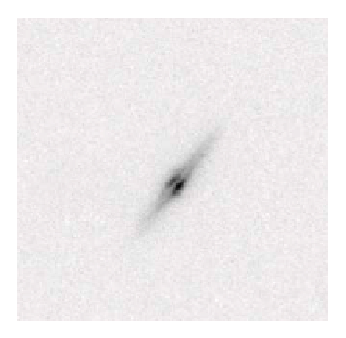
\includegraphics[width=5cm,height=5cm]{f1a.eps}
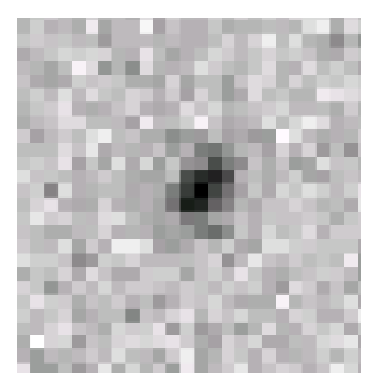
\includegraphics[width=5cm,height=5cm]{f1b.eps}
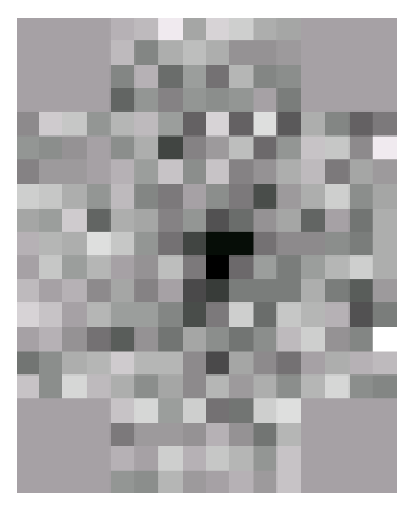
\includegraphics[width=5cm,height=5cm]{f1c.eps}
\caption{COSMOS image (left panel),
  SHERA simulated image (middle panel) and SDSS real image of the
  same galaxy (right panel).}
  \label{fig:image}
\end{figure*}

SHERA M12 is designed to test the accuracy of shape
measurement pipelines performing on ground-based images. It uses COSMOS
(Cosmological Evolution Survey) images as input, and the output
are low-resolution images expected from a given ground-based 
observation. Here we set parameters, such as pixel size, PSF size, 
and sky background, according to SDSS.  
The weak lensing shear signal is added to each image using the
following equation,
\begin{equation}
\left(
      \begin{array}{c}
               x^u\\
               y^u\\
       \end{array}
\right)=
\left(
      \begin{array}{cc}
               1-\kappa-\gamma_1 & -\gamma_2\\
               -\gamma_2 & 1-\kappa+\gamma_1\\
      \end{array}
\right)
\left(
\begin{array}{c}
               x^l\\
               y^l\\
       \end{array}
\right)\,,
\end{equation}
where $(x^u,y^u), (x^l,y^l)$ are the un-lensed coordinates and lensed
coordinates, respectively. The input shear $(\gamma_1, \gamma_2)$, 
are randomly generated ranging from -0.05 to 0.05.    

The input galaxy image catalog is constructed from COSMOS ACS 
field \citep{Koekemoer2007,Scoville2007a, Scoville2007b} following
the method described in \citet{Leauthaud2007}. The survey field is 
a $1.64$ square degree region centered at 
10:00:28.6$+$0.l2:12:21.0 (J2000).  The images are corrected 
for charge transfer inefficiency \citep[CTI]{Massey2010}, geometric 
distortion, sky subtraction and cosmic ray, and further dithered using 
multi-drizzle algorithm.  The final production has a co-added image of 
$7000\times 7000$ pixels with a scale of 0.03"/pixel.  Further cuts are 
applied to fulfill the special requirements of SHERA  as described in 
$\S 4.1$ of M12. 
%\begin{enumerate}
%\item $FW814<22.5$: This cut guarantees that the object observed in
%                 COSMOS can also be detected in SDSS. \\
%\item MU-CLASS=1: This selection \citep{Leauthaud2007} ensures a galaxy sample
%                free of stars, false detection due to residual cosmic rays.\\
%\item CLEAN: This step \citep[see also][]{Leauthaud2007} further eliminates galaxies with
%             defects caused by nearby bright stars, or other blending issues.\\
%\item GOOD-ZPHOT-SOURCE: This cut ensures the reliability of the measured photometric
%             redshift by avoiding SUBARU masked regions in B, V, I, z imaging.\\
%\end{enumerate}

 With the above criteria, 30,225 galaxies are selected.  To mimic
the SDSS images, additional galaxies are discarded either because 
these sources are undetectable in SDSS or because their sizes are smaller 
than the SDSS PSF, as detailed in M12. The final
sample contains 26,113 galaxies.

\subsubsection{PSF matching}

The high resolution images obtained above are transformed into low
resolution ones by PSF matching, i.e. by first de-convolving the 
images with the space PSF and then convolving them with the 
ground-based PSF.  In Fourier space, this is mathematically given by 
\begin{equation}
\tilde{I^g}=\frac{\tilde{G^g}}{\tilde{G^s}}\tilde{I^s}\,,
\end{equation}
where $I^g$ and $G^g$ are the ground-based brightness distribution
and PSF,  whereas $I^s$ and $G^s$ are the corresponding 
space-based quantities. This PSF matching works as long as 
the power spectrum of the space PSF is larger than that of the
ground PSF at all $k$; otherwise it leads to ringing effect in the
new image.  As shown in Fig.\,2 of M12, 
the power of SDSS PSF is smaller than that of COSMOS at all 
wave numbers, and so the PSF matching can be done safely.

In addition to the PSF, the noise level at the position of COSMOS in the
SDSS imaging should also be taken into account. Fig. \ref{fig:image} shows
the COSMOS image of a typical disk galaxy (left), SHERA simulated SDSS
image (middle) and the real SDSS fpAtlas image (right)
of the same galaxy. The bulge and disk components 
can be clearly identified from the original COSMOS image, 
whereas in SDSS only a bunch of pixels brighter than the detection limit 
(22.0 in r band) can be identified.  
We downgrade the high resolution COSMOS images to low 
resolution SDSS images. During this process, we miss 2.2 percent 
of the objects because of masking, which leaves a total of 25,527 
images.

\subsubsection{SHERA testing results}

\begin{figure}
\centering
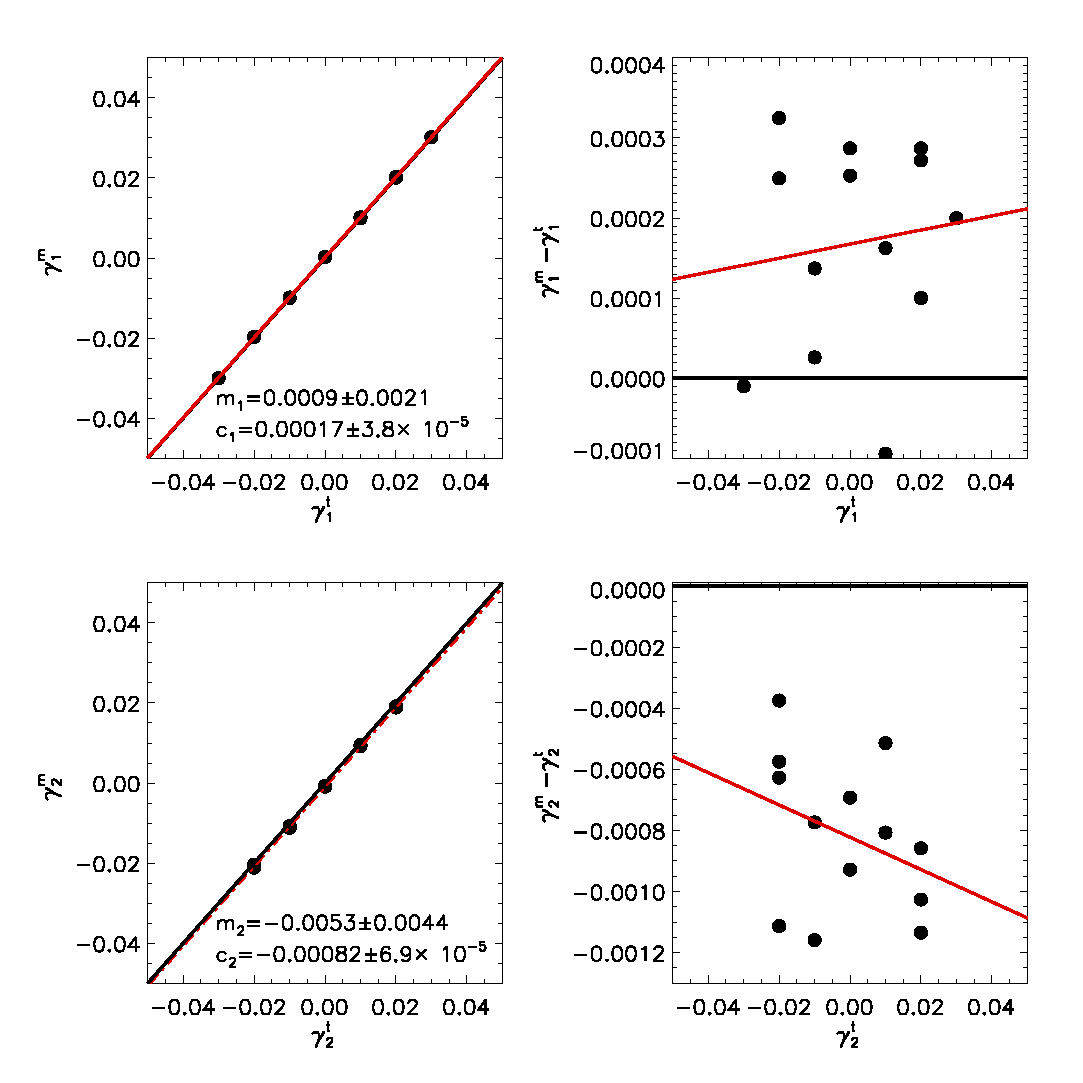
\includegraphics[width=8cm]{f2.eps}
\caption{The correlation between the true (input) and measured shear 
components $\gamma_1$ (upper left) and $\gamma_2$ 
(lower left). The corresponding residuals versus the input values 
are plotted in the right two panels. The red lines are linear fitting results.}
\label{fig:shera}
\end{figure}

Using the mock SDSS images obtained above, we follow
M12 to rotate each image 90 degree to eliminate the
effect from intrinsic shape of galaxies. Here, in order to have a fair
comparisons with the results of 12, 
the sky background and Poisson noise are not added to the simulation,  
so as to single out the performance of the PSF correction. 
Due to the size cut, only about 11,700 (44\%) galaxies are 
selected for the final shear measurement.

To quantify the performance of the pipeline, we measure the
shear, $\gamma$, in a given direction by averaging the shape of the 
source galaxies
\begin{equation}
\gamma=\frac{1}{2\textit{R}}\frac{\sum w_ie}{\sum w_i}\,, 
\end{equation}
where $e=(e_1, e_2)$ describes the image shape, $w_i$ 
is a weight assigned to an image, and  $R$ is the so called 
responsively calculated variance of the shape 
$\textit{R}=1-\langle e^2\rangle$.  
The shape parameters, $e_1$ and $e_2$, are obtained from 
the luminosity-weighted second moment of the 2-dimensional
galaxy image \citep{Kaiser1995}, 
\begin{equation}
M_{ij}=\frac{\sum G(x,y) I(x,y)(x-x_0)(y-y_0)}{\sum G(x,y)I(x,y)}\,,
\end{equation}
where $I(x,y)$ is the brightness at a certain pixel located 
at $(x,y)$, and $G(x,y)$ is a kernel to smooth the image.
Following convention, the ellipticities, $e_1$ and $e_2$, 
are defined to be compressions along a fiducial direction (e.g. $x$)
and along a direction that  is at 45 degree with respect to 
the fiducial direction, respectively. The weight $w_i$ for each 
galaxy is modeled as 
\begin{equation}
w=\frac{1}{\sigma_e^2+\sigma_{\rm sky}^2}\,, 
\end{equation}
where $\sigma_e$ is the variance of shape noise, 
and $\sigma_{\rm sky}$  describes the measurement error 
caused by the sky background and Poisson noise of photons. 

We measured the two shear components
$\gamma_1^{measure}$ and $\gamma_2^{measure}$, and 
Fig. \ref{fig:shera} shows the correlation between the measured signal
and input signal.  The upper-left and low-left panels are the one
correlations for the two components, while the right panels
are the corresponding residuals plotted against the input signal. 
The red lines are the linear fit to the data points.  
We use the standard terminology of multiplicative error (including PSF smearing
effect and other unknown bias due to measurement method itself) 
and additive error (mostly from PSF ellipticity a.k.a PSF anisotropy)
to connect the input signal and the measured signal:
\begin{gather}
\gamma_i^{measure}=(1+m_i)\gamma_i^{input}+c_i
~~~~(i=1,2)
\end{gather}
where $m_i$ and $c_i$ represent the two types of errors.  
In general, our pipeline achieves $<1\%$ in the multiplicative error, 
with $m_1=0.09\% \pm 0.0021$ and $m_2=0.53\%\pm 0.0044$, 
and $<0.1\%$ in the additive error, with  $c_1= 0.00017\pm
3.8\times 10^{-5}$ and $c_2= 0.00082\pm 6.9\times 10^{-5}$. 
The fact that the multiplicative error in $\gamma_2$ is larger 
than that in $\gamma_1$ is due to pixellization.  
In \citet{Mandelbaum2012} the corresponding multiplicative errors are
$m_1=-1.6\% \pm 0.001$ and $m_2=-2.7\% \pm 0.001$, and the 
additive errors are $c_1= 0.00028\pm 1.0\times 10^{-5}$ and 
$c_2 = -0.00011\pm 1.0\times 10^{-5}$.
The performance of our pipeline compares favorably 
to theirs. 

However, we did find  some shortcomings in our pipeline.  
When strong sky background and Poisson noise are added, 
our pipeline sometimes suffers from non-convergence problem 
either during the calculation of the adaptive moments or 
in the estimation of the coefficients in Eq. \ref{eq:kernel}.
Thus, our pipeline cannot provide shape measurements 
for images with too low qualities.  This reduces the number of 
sources that can be used for lensing studies. Due to the fact
that the COSMOS image sample is small, we do not perform further
test with noise as in M12. The convergence
problem is also not discussed in this work, because it is difficult
to examine weather it is from the iteration of adaptive moments or
in the procedure when constraining the $k_{ij}$.

Nevertheless, as  we will show in next subsection, even with the
reduced number of sources, our pipeline provides 
lensing signals that are competitive in comparison 
to other pipelines.

\subsection{GREAT3 }

GREAT3(GRavitational lEnsing Accuracy Test 03) 
\citep{Mandelbaum2014} is a successive testing project after
STEP \citep[Shear TEsting Program,][]{Heymans2005}, STEP2
\citep{Massey2007}, GREAT08 \citep{Bridle2009}, and GREAT10
\citep{Kitching2010}, all of which are designed to compare the 
performances of different shape measurement methods in different 
observational conditions. From STEP to GREAT3, different PSFs, 
pixel sizes, galaxy morphologies are adopted. In particular, 
GREAT3 uses controlled galaxy morphologies generated with 
Shapelets \citep{Refregier2003}, real galaxy morphologies obtained 
from COSMOS, co-added multiply observed images, variable PSF, 
and variable shears. Five major branches of simulations are 
generated using GalSim \citep{Rowe2015}:
(i) a controlled sample generated with parametric (single or double Sersic) 
galaxy models; (ii) real galaxy sample with realistic morphology 
from HST COMOS dataset; (iii) multiple-epoch sample containing six
images combined by dithering; (iv) sample with variable PSF 
that is reconstructed from star images;  (v) a sample that includes all the
above procedures.  Each branch has ground versus space, 
and constant versus variable shear sub-branches.

%For the constant shear branches, a $Q_\mathrm{c}$ matrix is 
%constructed from $m_i$ and $c_i$ ($i=1,2$) to rank the performance 
%of shape measurement methods:
%\begin{equation}
%Q_\mathrm{c}=\frac{1000\times \eta_\mathrm{c}}{\sqrt{\sigma_{\mathrm{min,c}}^2+
%\sum_{i=1,2}[(\frac{m_\mathrm{i}}{m_{\mathrm{target}}})^2+
%(\frac{c_\mathrm{i}}{c_{\mathrm{target}}})^2]}}\,,
%\end{equation}
%where $\sigma_{\rm min,c}$ is the typical dispersion in the
%quadratic sum of $m_i/m_{\mathrm{target}}$ and
%$c_i/c_{\mathrm{target}}$ due to pixel noise.
%Motivated by the estimated Euclid requirements \citep{Cropper2013, Massey2013}, 
%the normalizations are taken to be $m_{\mathrm{target}}=2\times 10^{-3}$ 
%and $c_{\mathrm{target}}=2\times 10^{-4}$. 
%The quantity $\eta_{\rm c}=1.232$ is a scale factor so that $Q\approx 1000$
%for methods meet the requirement of target $m_i$ and $c_i$. 
 
For the constant shear datasets, 10,000 galaxies with shear are
simulated. In order to cancel the effect of galaxy intrinsic shape,
GREAT3 applies the rotation method as in the STEP2 simulation
\citep{Massey2007}. The basic idea is to use the fact that the 
shape is a spin-two quantity for which the sum of the original ellipticity 
with that of the 90-degree rotation is zero.

Our pipeline participated in the  controlled ground constant, controlled space
constant, real ground constant and real space constant
tests. Overall, our pipeline ranks 15 among a total of 26 pipelines. 
As mentioned earlier, our pipeline suffers from non-convergence 
problem. Together with the size cut using the resolution factor in 
Eq.~(\ref{eq:eq_R}), only about 40\% galaxies are used in 
the competition.  Among our submissions, we found
that the best weighting for our pipeline is to take the inverse of
the shape noise and errors from ellipticity as in \citet[herefater
M05]{Mandelbaum2015}.  The more detailed
information and results about the GREAT3 competition can be found in
 M05.

\section{Application to the SDSS DR7}
\label{sec_application}

After the above tests, we processed the SDSS DR7 \citep{Abazajian2009}
$r$ band imaging data with our pipeline.  The SDSS \citep{York2000} 
consists of three imaging and spectroscopic surveys 
(Legacy, SEGUE, and Supernova), using a 2.5m telescope at Apache 
Point Observatory in Southern New Mexico. The SDSS
photometric camera has two TDI (Time-Delay-and-Integrate) CCD scanning
arrays \citep{Gunn1998}.  One is a $6\times 5$ CCD array, with each of
the CCD having $2048\times 2048$ pixels (24 $\mu m \approx 3 arcseconds$ 
on the sky) for five-band photometry, and the other is a 24 $2048\times
400$ CCD array used for astrometry and focus monitoring. The DR7
imaging data, with \textit{u}, \textit{g}, \textit{r}, \textit{i},
\textit{z} band information,  covers about 8423 square degrees 
of the LEGACY sky, with information for about 230 million distinct 
photometric objects, and about 3240 square degrees of SEGUE sky, 
with about 127 million distinct objects (including many stars at low
latitude). The total number of objects identified as galaxies is 
about 150 million.

\begin{figure}
\centering
\includegraphics[width=9cm,height=9cm]{f3a.eps}
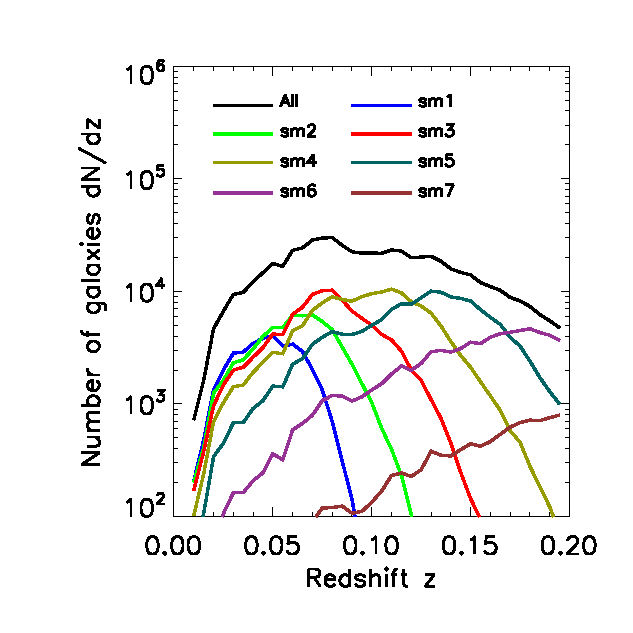
\includegraphics[width=9cm,height=9cm]{f3b.eps}
\caption{The redshift distribution of lens samples binned in
  luminosity (upper panel), and in stellar mass (lower panel).}
  \label{fig:zlens}
\end{figure}

\begin{table}[h!]
\begin{center}
 \caption{\label{tab:tbl-1} This table lists the six lens samples we
    selected and the corresponding numbers listed in
    \citet{Mandelbaum2005}}.
\begin{tabular}{ccccccc}
\hline
Sample & $M_r$ & $N_{gal}$ & $N_{M05}$ & $\langle z \rangle $ & $\sigma(z)$ & $\langle L \rangle/L_*$\\
\hline
L1  & $(-18,-17]$  & 18 614  & 6 524   & 0.029 & 0.007  & 0.071 \\
L2  & $(-19,-18]$  & 47 795  & 19 192  & 0.044 & 0.012  & 0.181 \\
L3  & $(-20,-19]$  & 138 988 & 58 848  & 0.069 & 0.020  & 0.450 \\
L4  & $(-21,-20]$  & 249 906 & 104 752 & 0.103 & 0.030  & 1.082 \\
L5  & $(-22,-21]$  & 164 653 & 63 794  & 0.140 & 0.038  & 2.364 \\
L6  & $(-23,-22]$  & 11 453  & 6 499   & 0.150 & 0.037  & 5.146 \\
\hline
\end{tabular}
\end{center}
\end{table}


\begin{table}[h!]
%\begin{center}
 \caption{\label{tab:tbl-2} This table lists some properties of the color
    divided sub-samples.}
\begin{tabular}{ccccc}
\hline
Sample & $N_{gal}$ & $\langle z \rangle $ & $\sigma(z)$ & $\langle L \rangle/L_*$\\
\hline
L1R   & 5 383   & 0.030  & 0.007  & 0.073 \\
L1B   & 13 231  & 0.029  & 0.007  & 0.071 \\
L2R   & 17 471  & 0.045  & 0.013  & 0.186 \\
L2B   & 30 324  & 0.044  & 0.012  & 0.179 \\
L3R   & 67 058  & 0.069  & 0.019  & 0.459 \\
L3B   & 71 930  & 0.069  & 0.019  & 0.443 \\
L4R   & 138 316 & 0.102  & 0.030  & 1.092 \\
L4B   & 111 590 & 0.104  & 0.030  & 1.072 \\
L5R   & 98 808  & 0.141  & 0.038  & 2.378 \\
L5B   & 65 845  & 0.138  & 0.038  & 2.347 \\
L6R   & 6 880   & 0.155  & 0.034  & 5.130 \\
L6B   & 4 573   & 0.141  & 0.037  & 5.182 \\
\hline
\end{tabular}
%\end{center}
\end{table}



\begin{table}[h!]
\begin{center}
 \caption{\label{tab:tb2-1} This table lists the seven lens samples we
    selected binned in stellar mass and the corresponding numbers listed in
    \citet[hereafter M06]{Mandelbaum2006}. Here and hereafter $M_*$ is presented in unit of
    $\msunhh$. }.
\begin{tabular}{ccccccc}
\hline
Sample & $\log(M_*)$ & $N_{gal}$ & $N_{M06}$ & $\langle z \rangle $ & $\sigma(z)$ & $\langle \log(M_*) \rangle$\\
\hline
sm1  & $[9.38,9.69]$    & 35 269  & 23 474   & 0.029 & 0.007  & 9.55 \\
sm2  & $[9.69,9.99]$    & 62 742  & 40 952   & 0.044 & 0.012  & 9.85 \\
sm3  & $[9.99,10.29]$   & 107 707 & 66 503   & 0.069 & 0.020  & 10.15 \\
sm4  & $[10.29,10.59]$  & 153 787 & 90 019   & 0.103 & 0.030  & 10.45 \\
sm5  & $[10.59,10.89]$  & 155 242 & 82 734   & 0.140 & 0.038  & 10.73 \\
sm6  & $[10.89,11.20]$  & 73 048  & 39 729   & 0.150 & 0.037  & 11.01 \\
sm7  & $[11.20,11.50]$  & 9 807   & 8 096    & 0.150 & 0.037  & 11.29 \\
\hline
\end{tabular}
\end{center}
\end{table}


\begin{table}[h!]
\begin{center}
  \caption{\label{tab:tb2-2} This table lists the sub samples binned
    in stellar mass and split into red and blue.}
\begin{tabular}{ccccc}
\hline
Sample & $N_{gal}$ & $\langle z \rangle $ & $\sigma(z)$ & $\langle \log(M_*) \rangle$\\
\hline
sm1r   & 7 447   & 0.038  & 0.010  & 9.56 \\
sm1b   & 27 522  & 0.054  & 0.016  & 9.55 \\
sm2r   & 19 604  & 0.051  & 0.015  & 9.87 \\
sm2b   & 43 138  & 0.070  & 0.020  & 9.85 \\
sm3r   & 48 669  & 0.069  & 0.019  & 10.16 \\
sm3b   & 59 038  & 0.089  & 0.026  & 10.15 \\
sm4r   & 85 839  & 0.090  & 0.025  & 10.45 \\
sm4b   & 67 948  & 0.113  & 0.032  & 10.44 \\
sm5r   & 102 360 & 0.120  & 0.036  & 10.74 \\
sm5b   & 52 882  & 0.136  & 0.037  & 10.72 \\
sm6r   & 57 063  & 0.149  & 0.037  & 11.01 \\
sm6b   & 15 985  & 0.146  & 0.038  & 10.99 \\
sm7r   & 8224    & 0.158  & 0.034  & 11.29 \\
\hline
\end{tabular}
\end{center}
\end{table}


\begin{table}[h!]
\begin{center}
  \caption{\label{tab:tb2-3} This table lists the sub samples binned
    in stellar mass and split into star forming galaxies and quenched
    galaxies.}
\begin{tabular}{lcccc}
\hline
Sample & $N_{gal}$ & $\langle z \rangle $ & $\sigma(z)$ & $\langle \log(M_*) \rangle$\\
\hline
sm1sf   & 29 460  & 0.053  & 0.016  & 9.55   \\
sm1qu   & 5 809   & 0.038  & 0.011  & 9.56   \\
sm2sf   & 46 544  & 0.068  & 0.020  & 9.85   \\
sm2qu   & 16 198  & 0.051  & 0.016  & 9.87   \\
sm3sf   & 66 138  & 0.086  & 0.027  & 10.15  \\
sm3qu   & 41 569  & 0.069  & 0.019  & 10.16  \\
sm4sf   & 73 606  & 0.109  & 0.031  & 10.44  \\
sm4qu   & 80 181  & 0.090  & 0.026  & 10.45  \\
sm5sf   & 50 107  & 0.137  & 0.034  & 10.72  \\
sm5qu   & 105 135 & 0.119  & 0.034  & 10.74  \\
sm6sf   & 11 151  & 0.157  & 0.033  & 10.98  \\
sm6qu   & 61 897  & 0.147  & 0.038  & 11.01  \\
sm7qu   & 8 219   & 0.157  & 0.034  & 11.29  \\
\hline
\end{tabular}
\end{center}
\end{table}


\begin{figure}
\centering
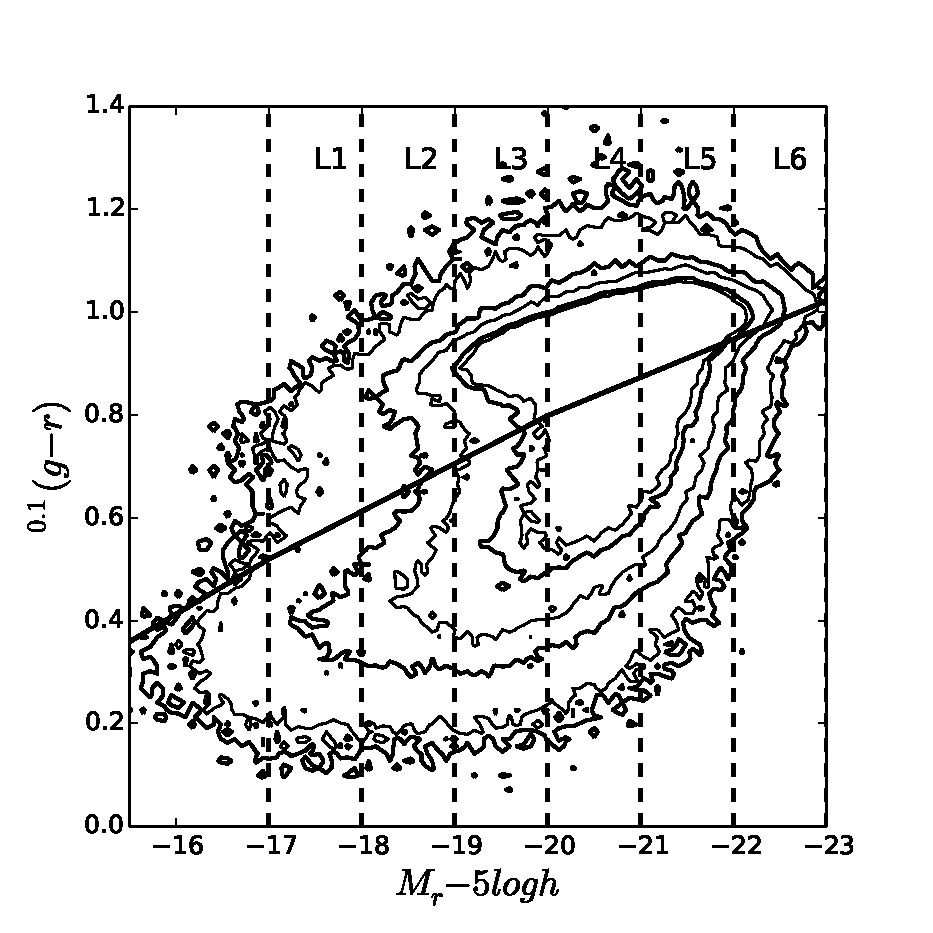
\includegraphics[width=7cm,height=7cm]{f4a.eps}
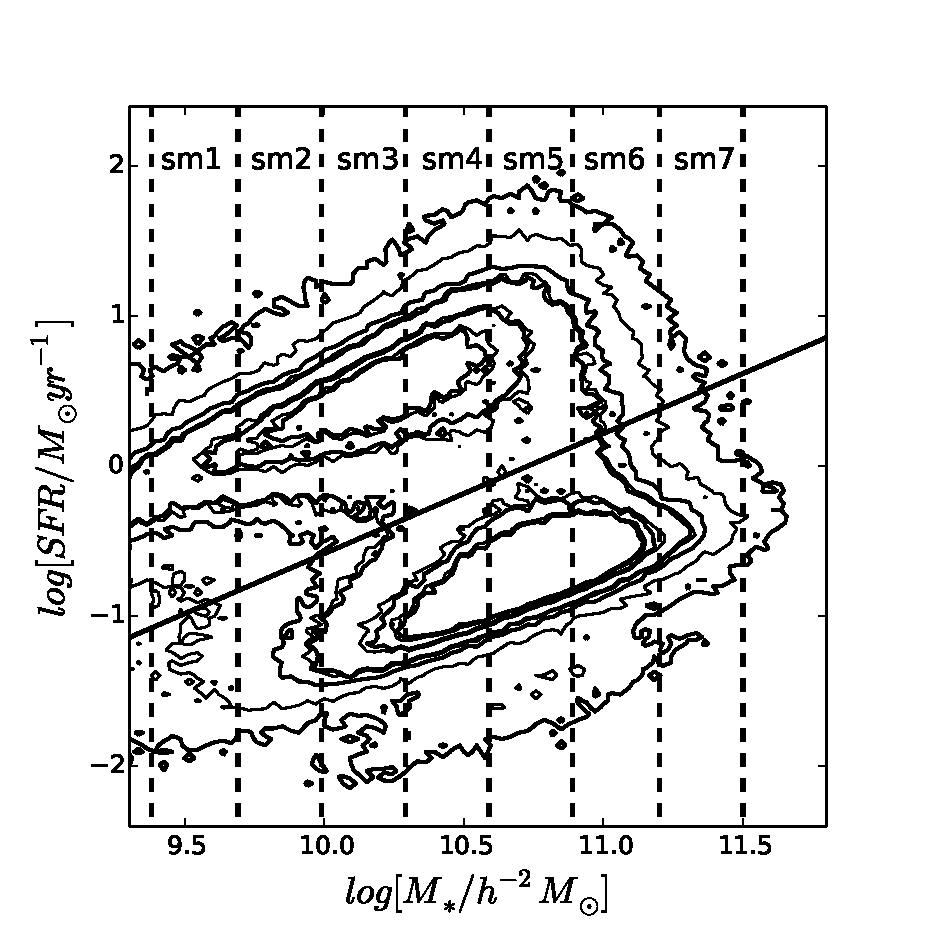
\includegraphics[width=7cm,height=7cm]{f4b.eps}
\caption{Upper panel: The distribution of lens galaxies in the 
color-absolute magnitude plane as represented contours.  The
luminosity bins used in the paper are shown as vertical dashed lines.
The solid line is the function used to divide red and blue galaxies 
\citep{Yang2008}.
Lower Panel: The distribution of lens galaxies in the 
star formation Rate (SFR)-stellar mass plane as represented 
by contours.  The stellar mass bins used in the paper are shown 
as vertical lines and the solid line is the function separating star forming 
galaxies from quenched galaxies \citep{Luo2014}.}
\label{fig:sublens}
\end{figure}

\subsection{Lens galaxies}

In modern galaxy formation paradigm, brighter or more massive galaxies
are believed to reside on average in more massive halos. This suggests
that the galaxy-galaxy lensing signals should vary with the 
luminosity or stellar mass of lens galaxies, in that 
brighter or more massive lens galaxy sample should give higher 
lensing signal. This expectation has been proved to be correct, as shown 
in e.g. M05, M06 and \citet{Sheldon2009}. In M05, lens galaxies 
in SDSS DR4 are divided into six luminosity samples, with the  
luminosity bins as given in Table. \ref{tab:tbl-1}. Here we use 
the same luminosity bins. We select lens samples from the 
New York University Value-Added Galaxy catalog 
\citep[NYU-VAGC]{Blanton2005} constructed from SDSS DR7 
\citep{Abazajian2009}.  All galaxies have been
extinction-corrected,  with apparent magnitude brighter 
than $r=17.72$, with redshifts in the range $0.01\leq z\leq 0.2$, 
and with spectroscopic redshift completeness $C_z>0.7$. 
The completeness $C_z$ is defined as the average percentage of 
the galaxies that have spectroscopic redshift in their local sky 
coverage. The resulting galaxy sample contains a total
of 639,359 galaxies in a sky coverage of 7,748 square degrees.

The selection criteria and galaxy numbers of our six lens
galaxy samples are listed in Table. \ref{tab:tbl-1}. The scatter of
the redshift distribution, the ratio between the mean luminosity
and the characteristic luminosity $L_*$ ($M_*=-20.44$, as 
given in \cite{Blanton2003}),  and the number galaxies contained 
in each sample are also listed in Table. \ref{tab:tbl-1}. 
On average, the number of galaxies in our sample is 2 to 3
time larger than the corresponding M05 sample, simply 
because DR7 covers a larger area than DR4 (7748 v.s. 
4783 square degrees). The mean redshift from our lens sample 
is slightly lower than that of M05, because M05 also used
lenses at $z>0.2$ while the redshift range of our sample is 
between $0.01$ and $0.2$. The redshift distributions of our lens 
samples are shown in Fig. \ref{fig:zlens}. The solid black line 
is for the total sample, while the colored lines are for 
the six luminosity samples, as indicated.

We further divide galaxies in each luminosity bin into blue and red
according to 
\begin{equation}
^{0.1}(g-r)=1.022-0.0652x-0.0031x^2 \,,
\label{eq:eq_color}
\end{equation}
where $x=\rmag + 23.0$ \citep{Yang2008}. The upper panel of 
Fig.\,\ref{fig:sublens} shows the distribution of the lens galaxies 
in the color-absolute magnitude plane, with the black dashed line 
showing the demarcation line (Eq. \ref{eq:eq_color}), and
the vertical lines marking the different luminosity bins we use.

In \citet[herefater M06]{Mandelbaum2006}, galaxy-galaxy 
lensing signals are measured for lens galaxies binned in stellar
masses. Here we make a similar analysis.  Note, however, 
that the stellar masses in M06 are estimated from spectra, as
described in \citet{Kauffmann2003}, while the stellar masses in 
our sample are estimated using the model described 
in \citet{Bell2003}. Table \ref{tab:tb2-1} lists some of the properties 
in different stellar mass bins, such as the number of galaxies in 
our samples in comparison to that in M06, the mean redshift,
the scatter in redshift, and the mean stellar mass.
We further divide galaxies in each stellar mass bin into 
red and blue samples using  Eq.\,(\ref{eq:eq_color}). 
Table \ref{tab:tb2-2} shows the number, mean redshift, scatter of the
redshift, and the mean stellar mass of the galaxies in each of the 
color samples. In general, the mean stellar mass of the red sample 
is larger than that of the corresponding blue sample by 0.01 to 0.02 dex.

In addition to the color separation, we also separate galaxies in
different stellar mass bins into star forming and quenched
subsamples. Here we use the \citet{Yang2013, Luo2014} scheme to 
define star forming and quenched galaxies, and the dividing line 
is defined to be
\begin{equation}
\log SFR=(\log M_* -2\log h -11.0)\times 0.8\,.
\label{eq:eq_sf_qu}
\end{equation}
The lower panel of the
Fig. \ref{fig:sublens} shows the distribution of galaxies in the SFR -
stellar mass plane, with the black dashed line showing the dividing line 
given above. Note that $M_*$ is presented in units of $\msunhh$.  Table
\ref{tab:tb2-3} lists the number, the mean redshift, the scatter of
the redshift, and the mean stellar mass of each subsample.  
For each mass bin,  the average stellar masses in the two  
subsamples are similar,  while the mean redshifts differ slightly 
in that a quenched sample has slightly higher mean redshift 
than the star forming sample.

\subsection{Source galaxies}

Following \citet[][hereafter M05]{Mandelbaum2005}, we only chose
galaxies defined as OBJC\_TYPE=3 from PHOTO pipe developed by
\citet{Lupton2001}. They have to be detected both in $r$ and $i$ bands
(with $r<22$ and $i<21.6$ in model magnitudes). We firstly create a
preliminary catalog (Cat I) from SDSS casjobs with 115,052,555
galaxies containing positions (including run, rerun, camcol, field,
obj, ra, dec), and photometric redshifts.

Then we process the Cat I to include more information such as, (i) sky
level in unit of photon-electron using the information of gain value
in $r$ band, (ii) the position of each galaxy in terms of CCD
coordinates in order to get the PSF from psField files, (iii) the SPA
value denoting the angle between the camera column position with
respect to north from fpC files. We define this catalog as Cat II
containing 91,941,657 galaxies. The missing 23,110,898 are caused by
the fact that we discard objects with -9999 value on zero-point,
extinction coefficient, airmass, sky in $r$ band, and only keep
galaxies with flags BINNED1 (detected at $\geq 5$), SATUATED=0 (do not
have satuated pixels), EDGE=0 (do not locate at the edge of the CCD),
MAYBE-CR=0 (not cosmic rays), MAYBE-EGHOST=0 (not electronic ghost
line) and PEAKCETER=0 (centroiding algorithm works well for this
object).

Then we use our pipeline to process the images from fpAtlas and
psField files to generate the final catalog (Cat III). Cat III
contains the information of position, redshift, ellipticity,
resolution factor and calibration errors of each galaxy. The errors
are estimated from both sky background and photon noise as described
by Eq. 11 and Eq. 12 in M05. We only keep objects with valid $e_1$,
$e_2$, resolution factor. As mentioned above, our pipeline will
abandon those galaxy images that have in-convergent values of
ellipticity.  From GREAT3 testing, about 40\% galaxies were excluded
due to this effect, and we further require that ${\cal R}>1/3$ which
tosses another 10\%-30\%(varies depending on different simulation sets.) 
or so. Here, our Cat III has a final number of
galaxies of 41,631,361, which is $\sim$45\% of the original Cat
II. The Irregularity image from SDSS photo-pipe($\sim$4\%), 
resolution cut($\sim$11\%), and
inconvergence problem($\sim$40\%) together reduce the
number of the final catalog by $\sim$55\%. 




\subsection{Galaxy-galaxy lensing signals}

From weak lensing shear measurements, we can estimate the excess
surface density (ESD) of the lens system, which is defined
as,
\begin{equation}
\Delta\Sigma(R)=\Sigma(\leqslant R)-\Sigma(R)\,,
\end{equation}
where $\Sigma(\leqslant R)$ and $\Sigma(R)$ are the mean surface mass
density inside a certain radius $R$ and at the radius $R$,
respectively. The tangential shear is related to this quantity via a
critical density,
\begin{equation}
\gamma_t(R)\Sigma_c=\Delta\Sigma(R)\,,
\label{eq:gamma_R}
\end{equation}
where the  critical density in a lensing system is,
\begin{equation}
\Sigma_c^{-1}=\frac{4\pi G}{c^2}\frac{D_lD_{ls}(1+z_l)^2}{D_s}\,.
\end{equation}
Here $D_s$, $D_l$ and $D_{ls}$ are the angular diameter distances of
the source, the lens and between the lens and the source,
respectively.


The mean excess surface density around a lens galaxy is specified by
the line-of-sight projection of the galaxy-matter cross correlation
function, $\xi_{\rm gm}(r)=<\delta(r)_{g}\delta(r')_{m}>$, so that
%
\begin{equation}
\label{sigatr}
\Sigma(R) = 2 \overline{\rho} \int_{R}^{\infty} \xi_{\rm gm}(r) 
{r \, \rmd r \over \sqrt{r^2 - R^2}}\,,
\end{equation}
%
and
%
\begin{equation}
\label{siginr}
\Sigma(\leq R) = \frac{4\overline{\rho}}{R^2} \int_0^R y\,\,dy\,
 \int_{y}^{\infty} \xi_{\rm gm}(r) {r \, \rmd r \over \sqrt{r^2 - y^2}}\,
\end{equation}
%
with $\overline{\rho}$ the average background density of the Universe.  Note
in both equations, we have omitted the contribution from the mean density of
the universe, as it does not contribute to the ESD.  


If taking photometric redshift error of source galaxies into account,
then it has to convolve with the error distribution (see M05),
\begin{equation}
\Sigma_c^{-1}(z_l,z_p)=\int p(z_s|z_p)\Sigma_c^{-1}(z_l,z_s)dz_s\,,
\end{equation}
where $z_l$, $z_p$, $z_s$ denote the spectroscopic redshift of the
lens galaxy, the photometric redshift of the source galaxy and the
spectroscopic redshift of the source galaxy. Because the spectroscopic
redshift of most of the source galaxies are not available, the
determination of $p(z_s|z_p)$ relies on other spectroscopic
surveys. In M05's results, they obtain the error
distribution by cross identify the subsample of their source galaxies
with other spectroscopic surveys such as DEEP2, COMBO-17.

%%% Luminosity Bins All-----------------------------------------------
\begin{figure}
\centering
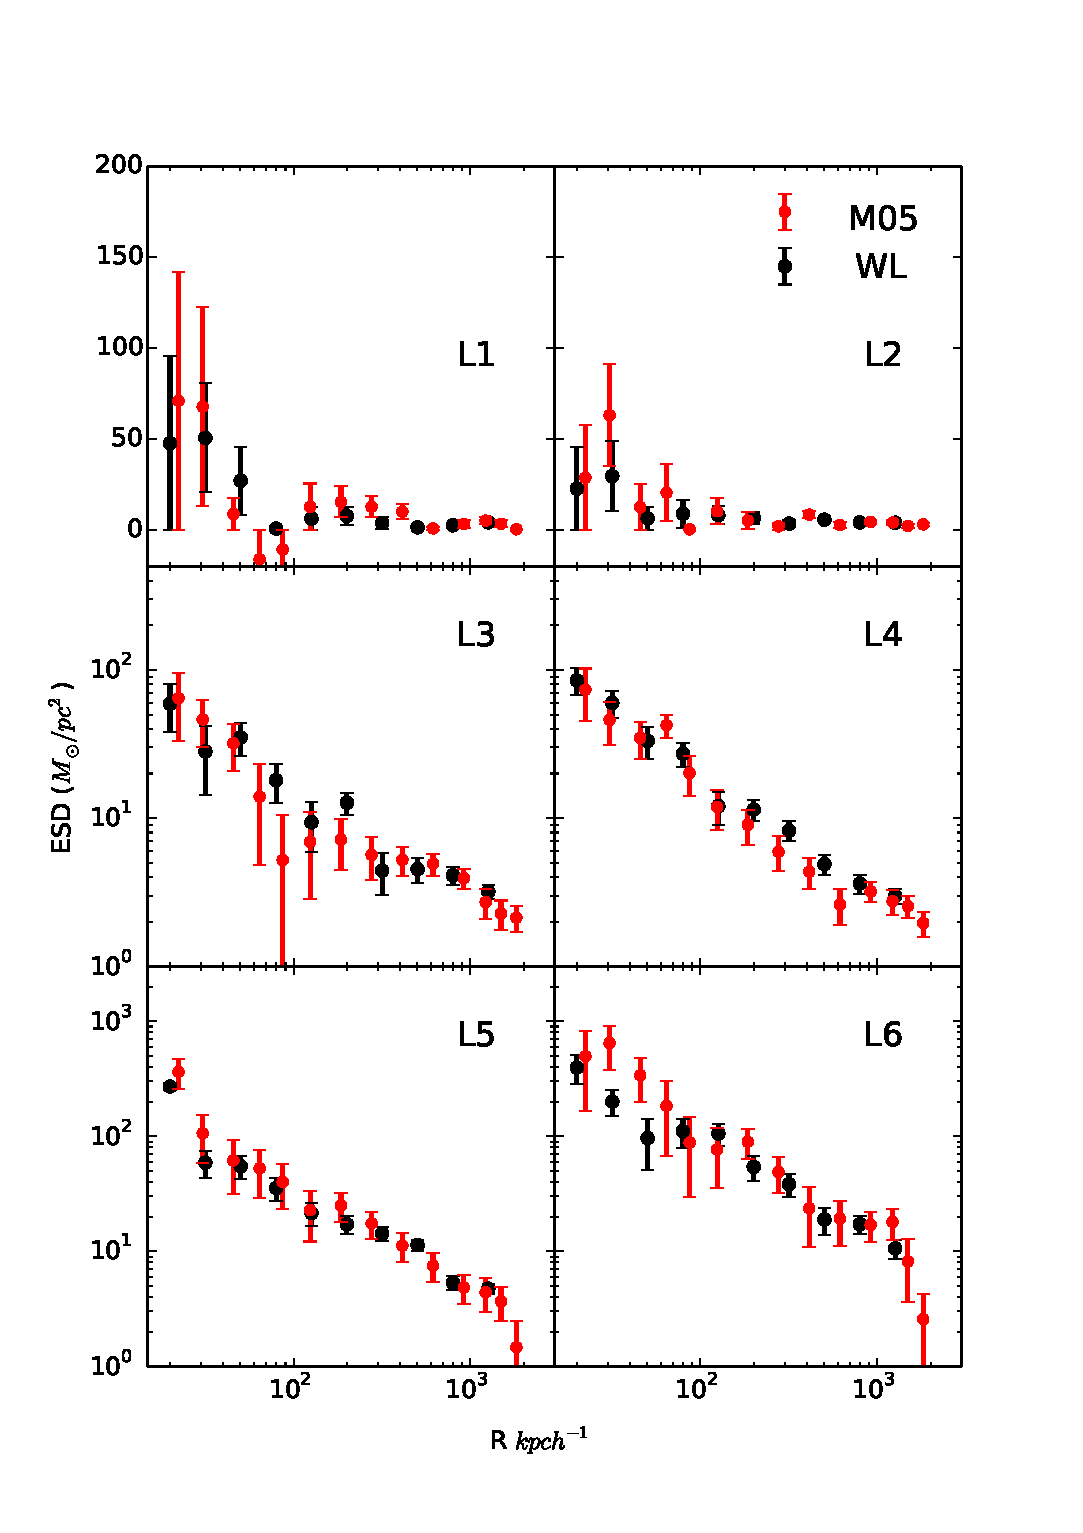
\includegraphics[width=7cm,height=9cm]{f5.eps}
\caption{The excess surface density (ESD) of our lens galaxies in six
  luminosity bins. The black dots are our measurements and the red
  dots are results obtained by M05.}
  \label{fig:compare_L}
\end{figure}


\begin{figure}
\centering
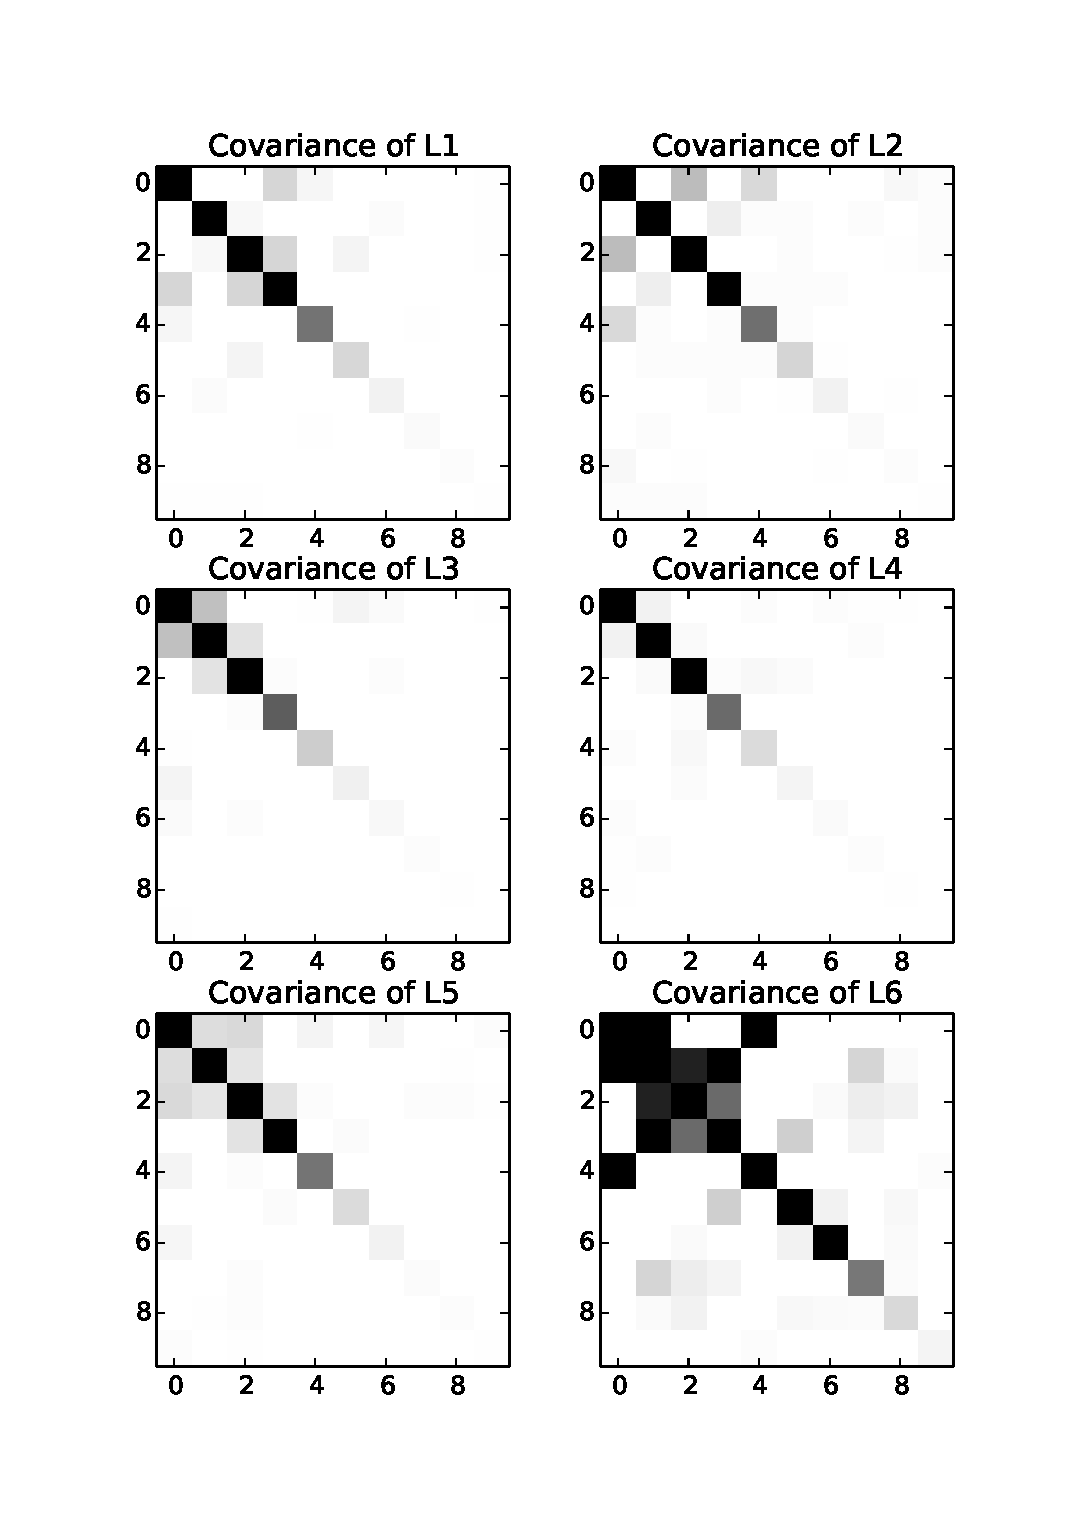
\includegraphics[width=7cm,height=9cm]{f6.eps}
\caption{The covariance matrix of the data points for our six
  luminosity bins. The grey scale color has been re-scaled so that
  smaller values can be reflected on this covariance map.  The values
  of the covariance map are provided in extra files. }
  \label{fig:covar_L}
\end{figure}

Fig. \ref{fig:compare_L} shows the average excess surface density of
our lens galaxies divided into six luminosity bins. The black dots are
our measurements and the red dots are kindly provided by Rachel
Mandelbaum. For simplicity we calculate the signals around each galaxy
sample in 10 equal logarithmic bins rather than 45 bins and re-bin the
signal as in M05. The error bars are estimated from 2500 bootstrap
resampling of the lens galaxies. Thus the related error bars shown in
the figure are mainly from the sampling variance.  The covariance
matrix of the data points shown in Fig.  \ref{fig:compare_L} are given
in Fig.  \ref{fig:covar_L}.  We rescaled the color so that smaller
values can be seen. For those who are interested, the covariance
values can be obtained via the link provided at the end of section
\ref{sec_intro}.

Following M05, we give a detailed list of possible systematic errors
that the measured signals might have in Appendix \ref{sec_systematic}.
The total $2\sigma$ systematic error in $\delta \gamma/\gamma$ is
about $[-9.1\%,20.8\%]$, slightly larger than those quoted in M05 at
about $[-9.0\%,+18.4\%]$ due to the fact that we directly use the
value from M05 of sample with $r>21.0$ to estimate the systematic.  In
addition, the redshift tests and $\gamma_{45}$ component tests are
consistent with zero.  Overall, our results are in very good agreement
with M05 ones with smaller error bars, which is due to the larger
number of lens galaxies in our samples. Both signals show clear
increasing trend as the luminosity increases.


%%% Luminosity Bins Red and Blue-------------------------------------------
\begin{figure}
\centering
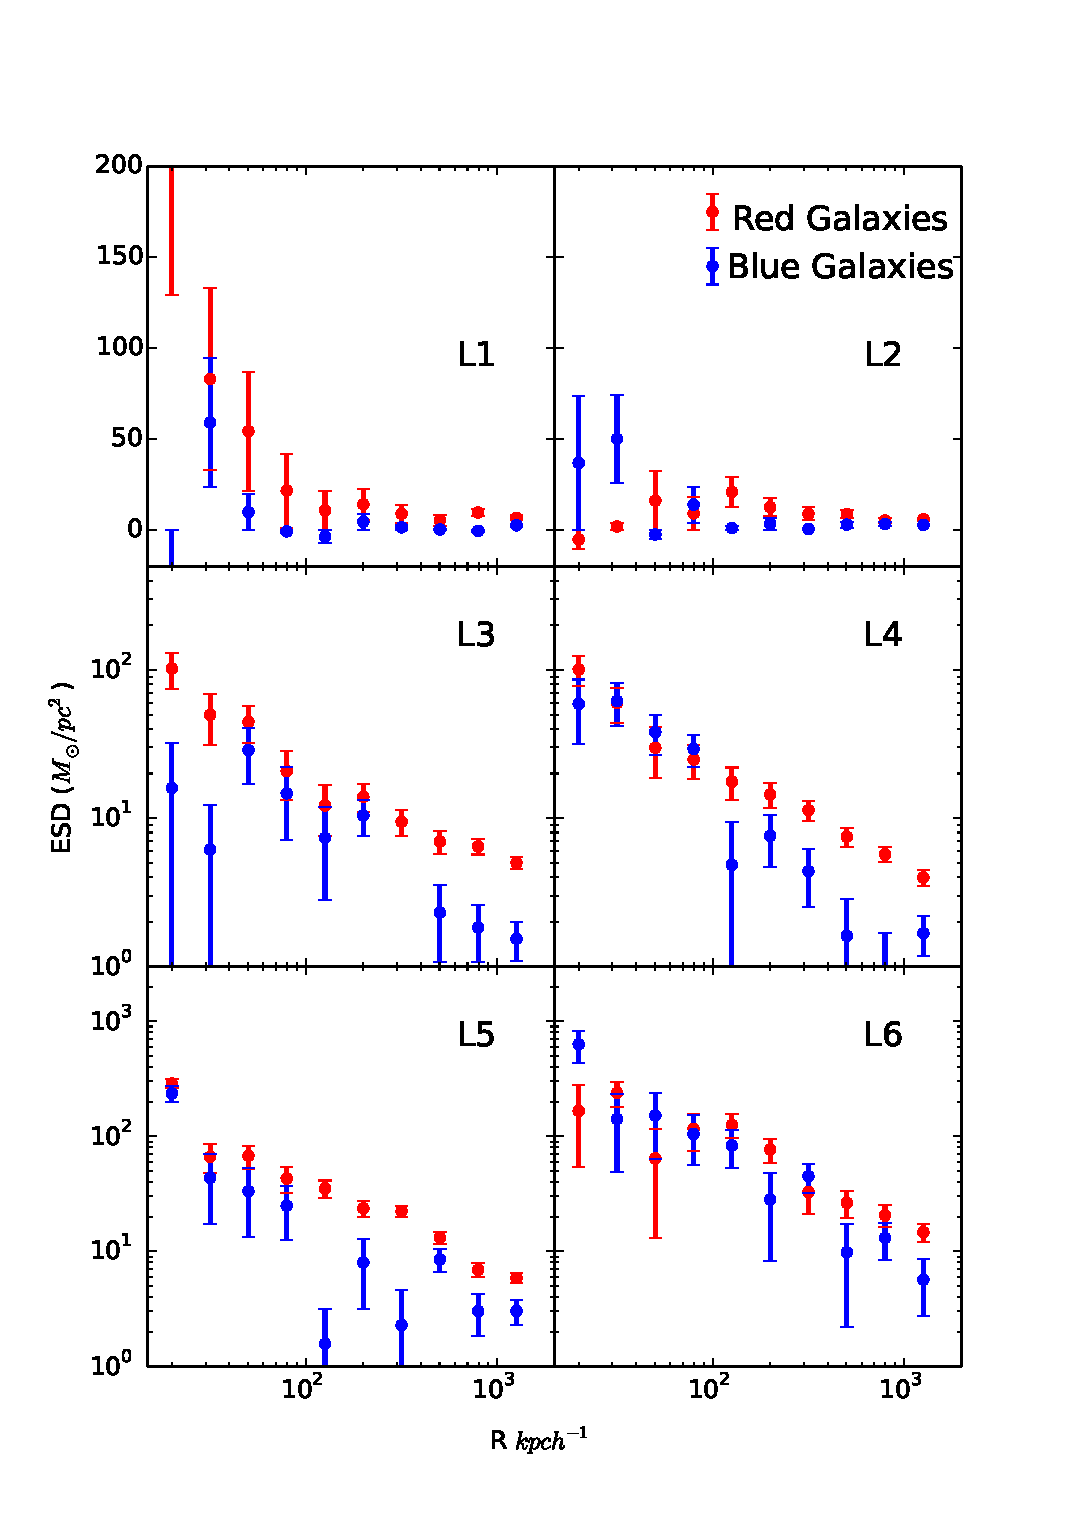
\includegraphics[width=7cm,height=9cm]{f7.eps}
\caption{The ESDs for  red (red dots) and blue (blue dots) galaxies in
  different luminosity bins.}
  \label{fig:Lbin_color}
\end{figure}





For each of our luminosity bin, we have divided galaxies into red and
blue subsamples, we show the corresponding galaxy-galaxy lensing
signals in Fig.  \ref{fig:Lbin_color}. The error bars become larger
due to the decreased number of lens galaxies in the subsamples. For
very faint lens galaxies in L1 bin, the red galaxies have larger ESDs
than blue galaxies especially at small radius, indicating that red
galaxies on average locate in relatively more massive halos than their
blue counterparts.  For relatively bright galaxies, especially in
L2-L4 bins, the red galaxies show similar ESDs as blue ones at small
scales, while at larger scales with $R> 200 \kpch$, the signals from
red galaxies are much larger than the blue galaxies. The much more
enhanced ESDs for red galaxies at large scale indicate that these
galaxies may locate in or near massive host halos.




%%% Stellar Mass Bins Red and Blue-----------------------------------------------

\begin{figure}
\centering
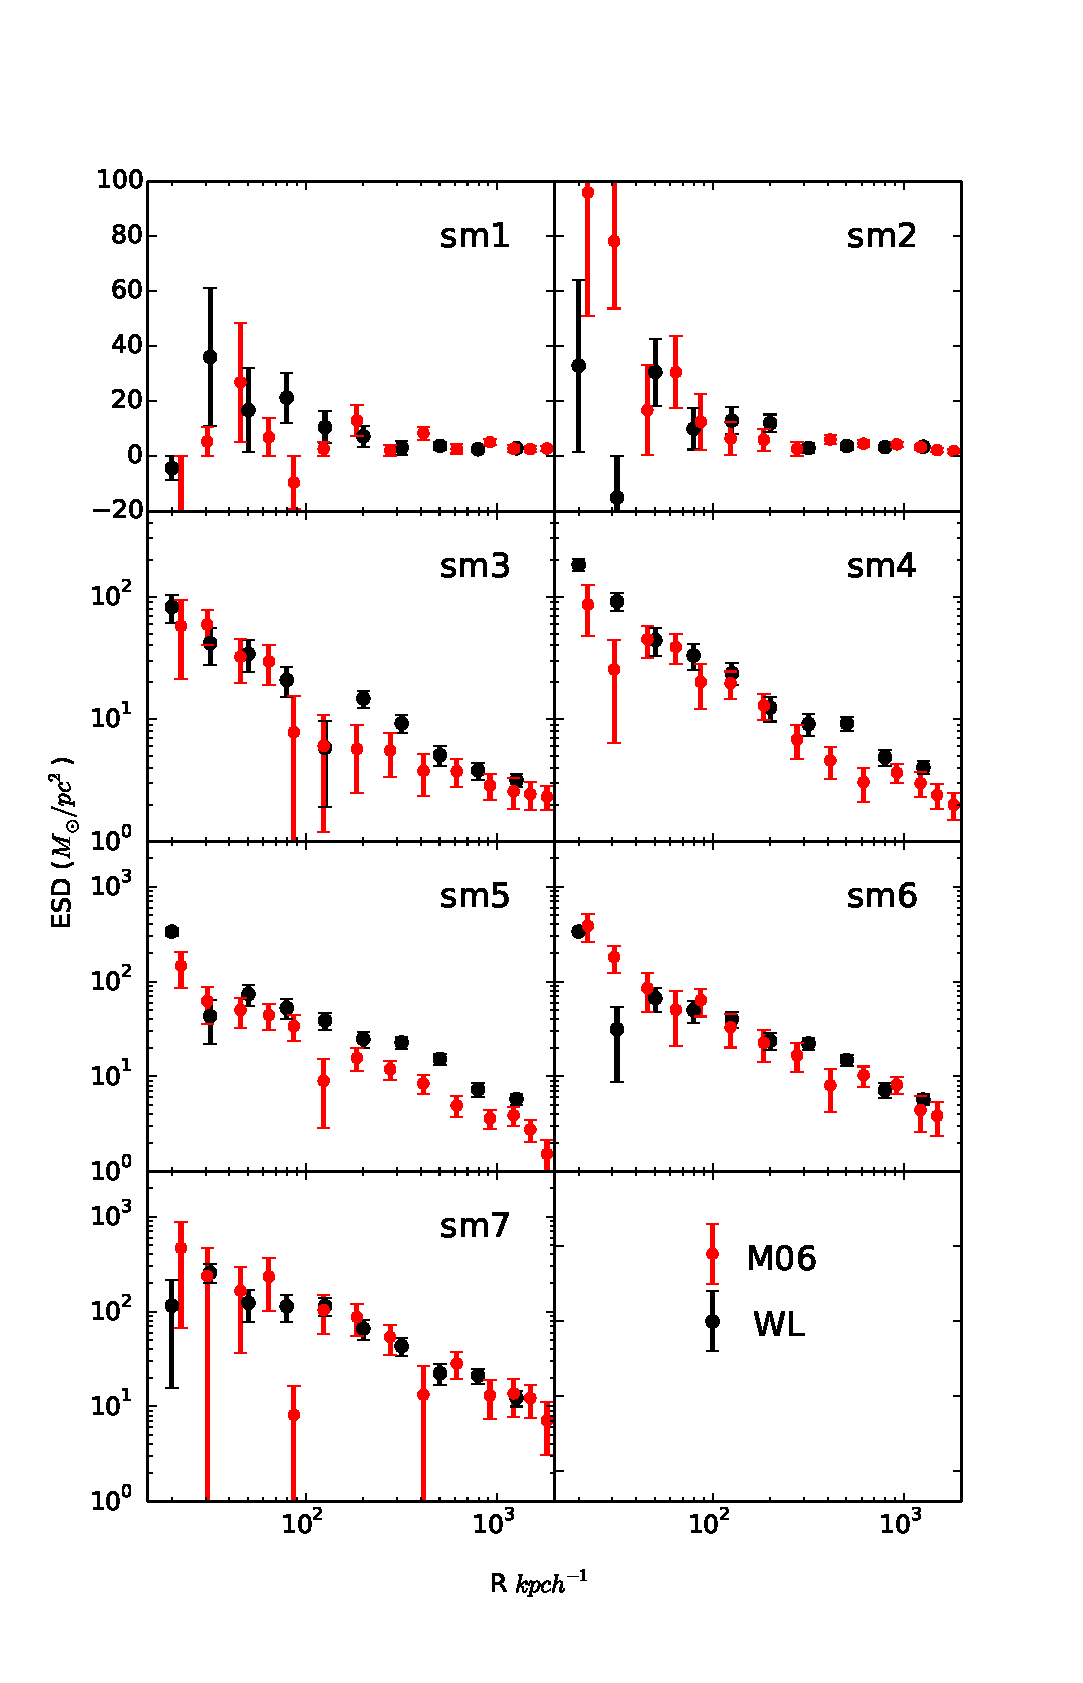
\includegraphics[width=7cm,height=9cm]{f8.eps}
\caption{The ESDs for lens galaxies that are separated into different
  stellar mass bins. Here in each panel we compare the results between
  our sample (black dots) and M06 (red dots). }
  \label{fig:compare_sm}
\end{figure}

%\begin{figure}
%\centering
%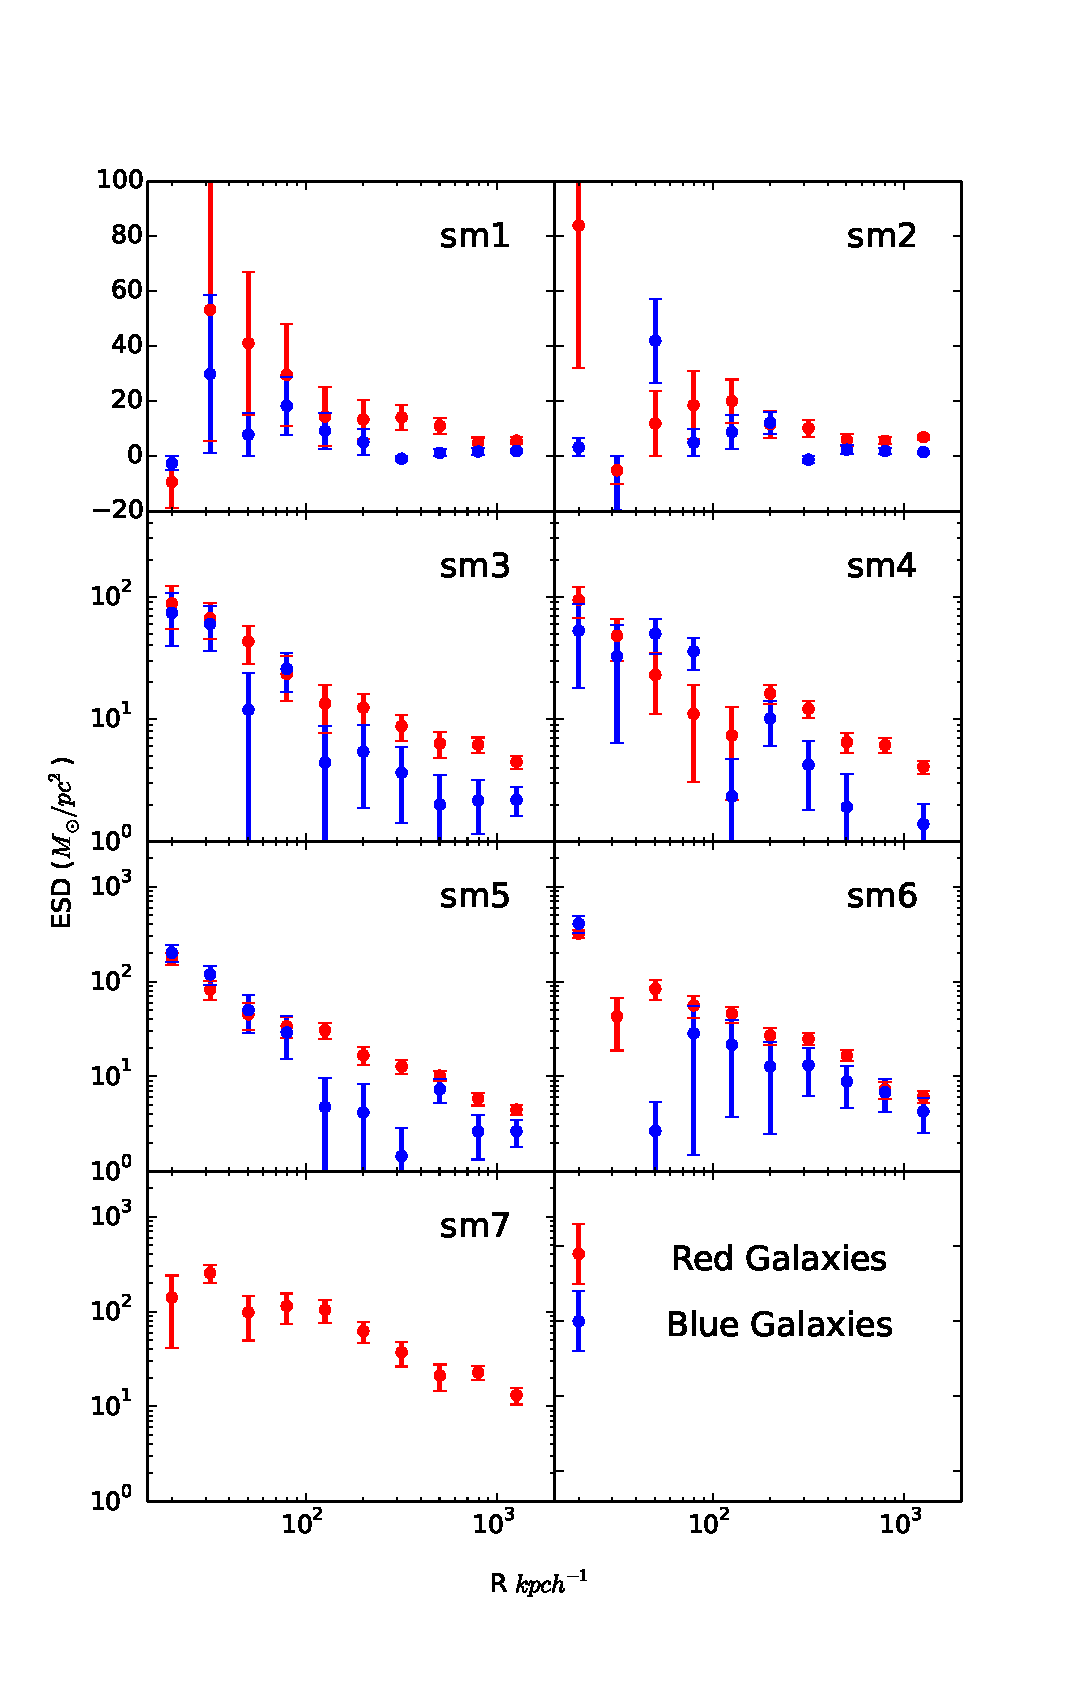
\includegraphics[width=7cm,height=9cm]{f9.eps}
%\caption{The covariance matrix of the data points for stellar mass
% bins. The same re-scale is applied as the luminosity binned sample
% so that smaller values can be seen.}
 % \label{fig:covar_sm}
%\end{figure}


Next, we proceed to estimate the ESDs for galaxies that are separated
into different stellar mass bins. Shown in Fig. \ref{fig:compare_sm},
the black dots are our measurements and the red dots are those
obtained by M06. Similar to the luminosity separation, our results
agree with those of M06 very well, except in the sm5 bin where ours
show enhanced ESDs at radius $1500 > R > 200 \kpch$. This enhancement
indicate that the additional galaxies in this sample relative to M06
may have a larger portion in or near massive halos.



%%% Stellar Mass Bins SF and QU------------------------------------------------------

\begin{figure}
\centering
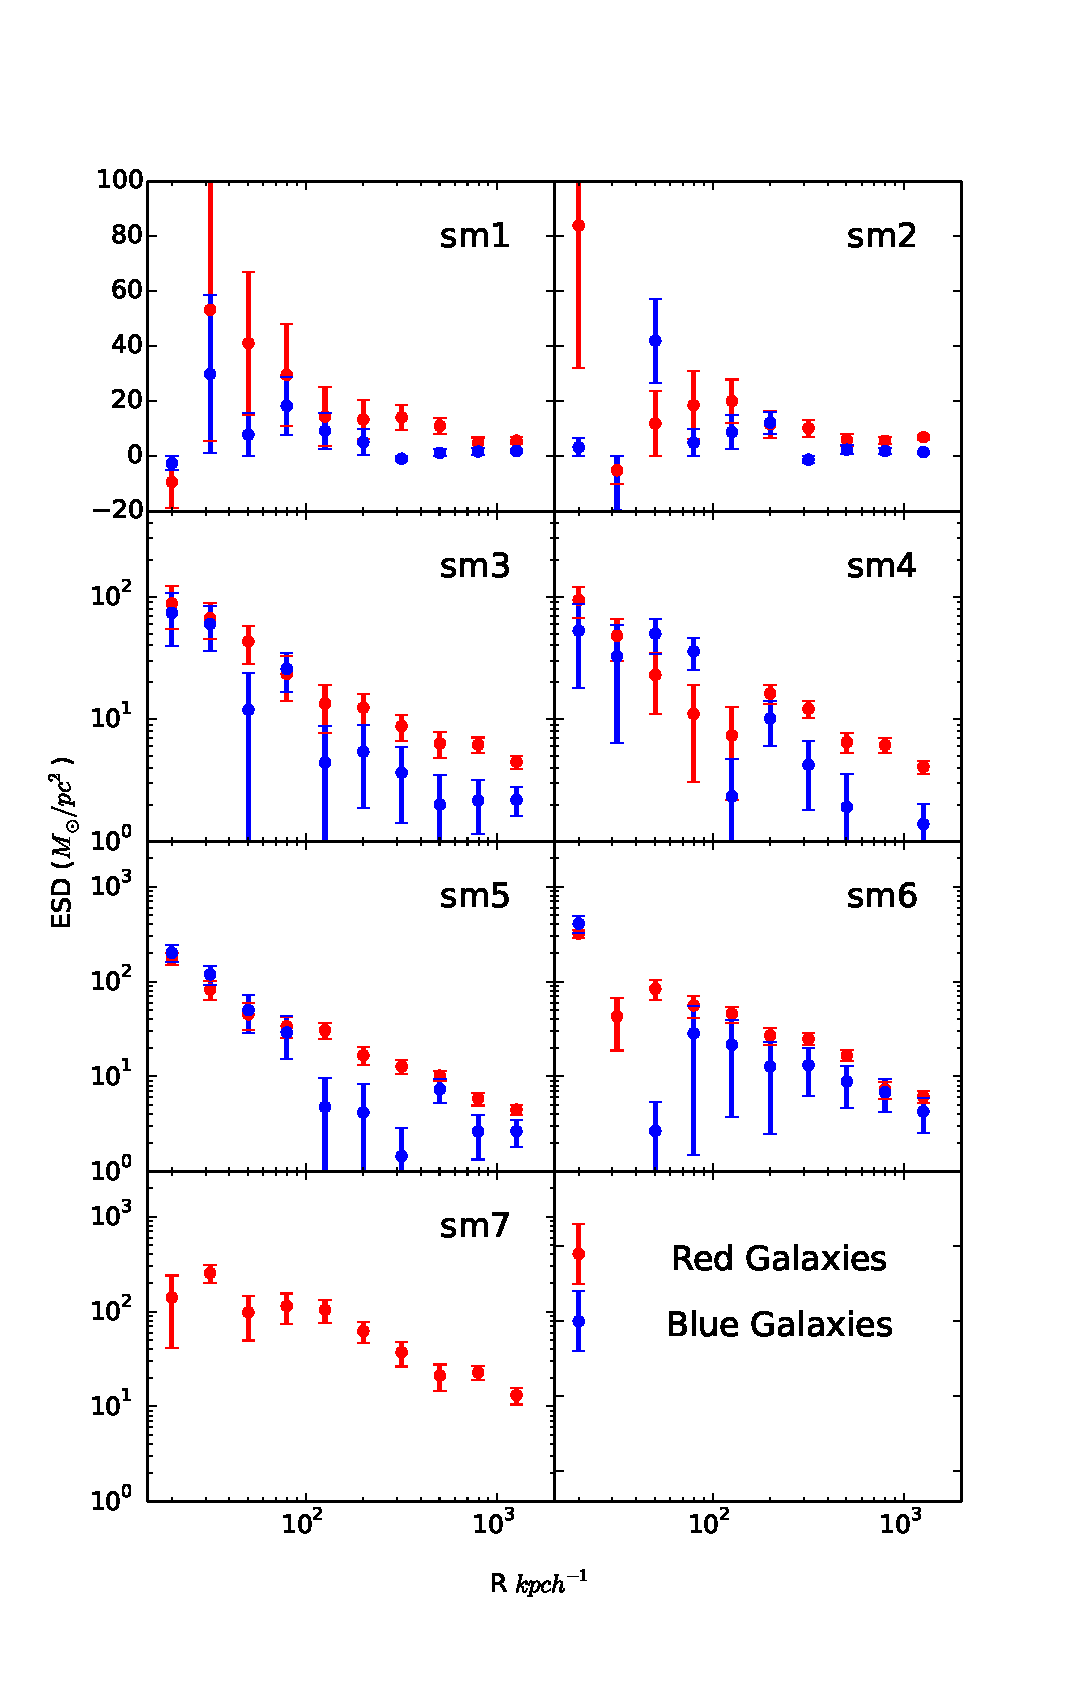
\includegraphics[width=7cm,height=9cm]{f9.eps}
\caption{The ESDs for red (red dots) and blue (blue dots) lens
  galaxies in  different stellar mass bins.}
  \label{fig:sm_color}
\end{figure}

\begin{figure}
\centering
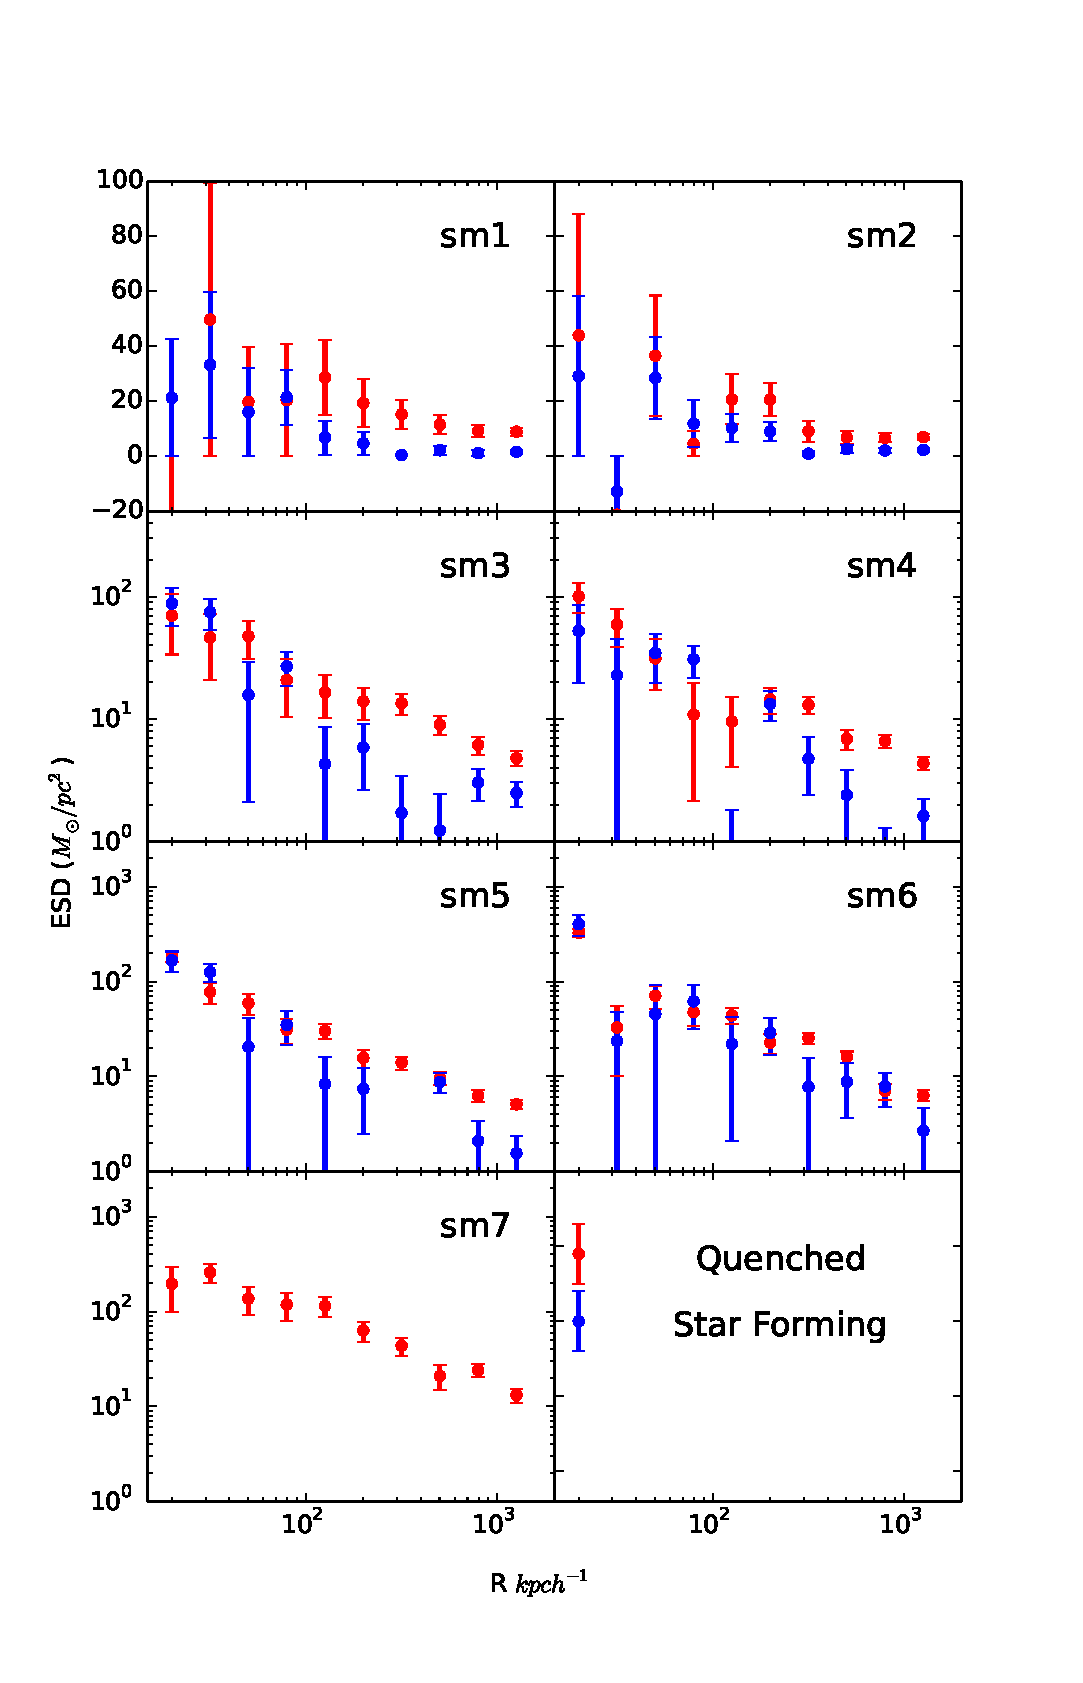
\includegraphics[width=7cm,height=9cm]{f10.eps}
\caption{The ESDs for quenched (red dots) and star forming (blue dots)
  lens galaxies in different stellar mass bins.}
  \label{fig:sm_sq}
\end{figure}




To be complete, we also measure the ESDs for our color and star
formation subsamples in different stellar mass bins. Shown in
Fig. \ref{fig:sm_color} are the results for red and blue galaxies. The
color dependences in different stellar mass bins are quite similar to
those in different luminosity bins. In addition, as the color are
closely related with the newly formed stars, i.e. young galaxies are
bluer whereas old galaxies are redder. Thus the results shown in
Fig.\ref{fig:sm_sq} for star forming and quenched galaxies are similar
to red galaxies.


Finally, as modelled in M05, the above measured ESD signals can be
fitted to probe the average halo mass of the lens systems. Also as
pointed out in \citet{Yang2006a}, the central and satellite galaxies
have very different lensing signals, we differ a more detailed
modeling of the ESDs on these lens galaxies in a subsequent paper
by separating them into central and satellite galaxies. 
 



\section{Discussion and Conclusion}
\label{sec_summary}

In weak lensing studies, to obtain a reliable measurement of the
lensing signals requires high accuracy of image processing. In this
paper, we build our image processing pipeline to achieve accurate
shape measurement for weak lensing study based on BJ02 and HS03
method. The basic performance of our pipeline is summarized as
follows.
%
\begin{itemize}
\item This pipeline is tested using SHERA and GREAT3 simulations.
  Tests show that our pipeline works well on PSF correction in the
  absence of sky background noise, the corrected PSF multiplicative
  errors are far below 1\% requirements ($0.009\%$ for $\gamma_1$ and
  $-0.053\%$ for $\gamma_2$) for PSF correction only.

\item For more realistic simulations with sky background noise, our
  pipeline skips about 40\% galaxies that might caused by the
  inconvergence problem of the method. In addition, to have a
  sufficient image resolution ${\cal R}>1/3$ will remove additional
  30\% galaxies. However, using the remaining galaxy images still
  helps us to obtain similar lensing reconstruction accuracy as most
  of the other methods as shown in GREAT3 results paper\citep{Mandelbaum2015}.

\item We applied our pipeline to the SDSS DR7 $r$ band imaging data
  and create a catalog containing 41,631,361 galaxies with the
  information of position, photometric redshift, ellipticity and
  ellipticity measurement error due to sky background and Poisson
  noise.

\item Using these galaxy images, we calculated the galaxy-galaxy
  lensing signals around foreground lens galaxies binned in different
  luminosities and stellar mass ranges. Comparing to those of M05 and
  M06, our results show very good agreement with these previous
  studies with significantly reduced error bars. The systematic checks
  using $\gamma_{45}$ components, redshift tests and random sample
  tests show null signals. These consistencies further confirmed the
  reliability of our pipeline.

\item We have also separate the galaxies in different luminosity or
  stellar mass bins into red/blue or star forming/quenched
  subsamples. The galaxy-galaxy lensing signals show quite different
  scale dependence among these subsamples.
\end{itemize}
%

As this is the first paper in a series on galaxy-galaxy lensing
studies, here we focused on testing the reliability of our image
processing pipeline. In the upcoming work, we will use the shape
catalog obtained from SDSS DR7 to study galaxy-galaxy lensing signals
around galaxy groups obtained by \citet{Yang2007, Yang2012} by
separating lens galaxies into central and satellite subsamples, etc.

On the other hand, as our pipeline can not make full use those images
that suffered significantly from the strong noises, we intend to
improve the pipeline by combining the Fourier space based method
\citep{Zhang2015}.  As pointed out in \citet{Zhang2015}, the Fourier
space based method is indeed very powerful in dealing with asymmetric
systems and those images that are strongly suffered from the noise.


\acknowledgements

WL hereby thank Rachel Mandelbaum from Carnegie Mellon University for
very useful guiding and discussions at various stages in carrying out
this project and providing the data points presented in this paper,
Dandan Xu from Heidelberg University for useful discussion.  This work
is supported by the 973 Program (No. 2015CB857002), NSFC
(Nos. 11128306, 11121062, 11233005, 11503064), the Strategic Priority
Research Program ``The Emergence of Cosmological Structures" of the
Chinese Academy of Sciences, Grant No.  XDB09000000, and a key
laboratory grant from the Office of Science and Technology, Shanghai
Municipal Government (No. 11DZ2260700) as well as Chinese Scholarship
Council(201504910477) and Shanghai Natural
Science Foundation, Grant No. 15ZR1446700. LF acknowledges support
from NSFC grants 11103012 \&11333001 \& Shanghai Research grant
13JC1404400. LR acknowledges the NSFC(grant No.11303033), 
the support from Youth Innovation Promotion Association of CAS.

This work is also supported by the High Performance Computing Resource
in the Core Facility for Advanced Research Computing at Shanghai
Astronomical Observatory.



%%%%%%%%%%%%%%%%%
% Appendix
%%%%%%%%%%%%%%%%%

\appendix

\section{A. BJ02 Method}
\label{bj02_detail}

In order to construct the basic components for $K$ as well as the
 corresponding coefficients of individual components. Eqs.\,(7.18) - (7.22) 
in BJ02 list the $3\times 3$ basic kernel components constructed on the
basis of flux conservation.  Flux conservation requires that the kernel is  
the sum of an identical matrix with the derivative matrices whose elements 
summation is zero. The continuous form of D is:
\begin{gather}
D_{ij}=(\frac{\partial}{\partial x}+i\frac{\partial}{\partial y})^i
       (\frac{\partial}{\partial x}-i\frac{\partial}{\partial y})^j\\
       =\sigma^{-(i+j)}(a_q^{\sigma\downarrow}-a_p^{\sigma\uparrow})^i(a_p^{\sigma\downarrow}-a_q^{\sigma\uparrow})^j.
\end{gather}
Here $a_{p}^{\downarrow}$ and $a_{p}^{\uparrow}$ are defined as
lowering and raising operators for 2D QHO eigenfunctions, which have
the properties
\begin{gather}
a_{p}^{\downarrow}=\frac{1}{2}[\frac{x-iy}{\sigma}+\sigma(\frac{\partial}{\partial x}-i\frac{\partial}{\partial y})],\\
a_{p}^{\uparrow}=\frac{1}{2}[\frac{x+iy}{\sigma}-\sigma(\frac{\partial}{\partial x}+i\frac{\partial}{\partial y})],\\
a_{q}^{\downarrow}=\frac{1}{2}[\frac{x+iy}{\sigma}+\sigma(\frac{\partial}{\partial x}+i\frac{\partial}{\partial y})],\\
a_{q}^{\uparrow}=\frac{1}{2}[\frac{x-iy}{\sigma}-\sigma(\frac{\partial}{\partial x}-i\frac{\partial}{\partial y})].
\end{gather}
The derivative along $x$ and $y$ axis can be treated as convolving a matrix with the image $I(x,y)$. 
\begin{gather}
\frac{\partial I}{\partial x}=\begin{pmatrix}0 & 0 &
0\\ \frac{-1}{2} & 0 & \frac{1}{2} \\0 & 0 & 0\end{pmatrix}\otimes I,\\
\frac{\partial I}{\partial y}=\begin{pmatrix}0 & \frac{1}{2} &
0\\ 0  & 0 & 0\\0 & \frac{-1}{2} & 0\end{pmatrix}\otimes I,\\
\frac{\partial^2 I}{\partial x^2}=\begin{pmatrix}0 & 0 &
0\\ 1  & -2 & 1\\0 & 0 & 0\end{pmatrix}\otimes I,\\
\frac{\partial^2 I}{\partial y^2}=\begin{pmatrix}0 & 1 &
0\\ 0  & -2 & 0\\0 & 1 & 0\end{pmatrix}\otimes I,\\
\frac{\partial^2 I}{\partial x \partial y}=\begin{pmatrix}\frac{-1}{4} & 0 &
\frac{1}{4}\\ 0  & 0 & 0\\ \frac{1}{4} & 0 & \frac{-1}{4}\end{pmatrix}\otimes I.
\end{gather}
These are the components of the Second Derivative
in the Gradient Direction(SDGD) filter in image edge detection.

In descrete form, the $3\times 3$ basic kernel are:
\begin{align}
D_{10}=\begin{pmatrix}0 & i(1/2) &
0\\ -1/2 & 0 & 1/2\\0 & i(-1/2) & 0\end{pmatrix}; D_{01}=\overline{D_{10}},\\
D_{20}=\begin{pmatrix}i(-1/2) & -1 &
i(1/2)\\ 1 & 0 & 1\\i(1/2) & -1 & i(-1/2)\end{pmatrix}; D_{02}=\overline{D_{20}},\\
D_{11}=\begin{pmatrix}0 & 1 &
0\\ 1 & -4 & 1\\0 & 1 & 0\end{pmatrix}.
\end{align}
The $D_{00}$ is the idential matrix. $D_{11}$ is an actually Laplacian operator. 
They contains all the first and second order derivatives.
Higher order derivatives can be found by convolving $3\times 3$
components. Then the kernel bears the following form
\begin{equation}
K=\sum k_{ij}D_{ij},
\label{eq:kernel}
\end{equation}
where $k_{ij}$ are the coefficients satisfying
$k_{ij}=\overline{k_{ij}}$ so that $K$ is a real matrix rather than
a complex one.


Combining equations \ref{eq4} and \ref{eq:kernel} we have
\begin{equation}
\mathrm{b}^{*}=\sum_{ij}k_{ij}D_{ij}\mathrm{b},
\end{equation}
where $D_{ij}\mathrm{b}$ obeys the recursion:
\begin{gather}
\label{eq:recursive}
D_{00}\mathrm{b}=\mathrm{b},\\
D_{(i+1)j}\mathrm{b}=\frac{1}{\sigma}(a_{q}^{\downarrow}-a_{p}^{\uparrow})D_{ij}\mathrm{b},\\
D_{i(j+1)}\mathrm{b}=\frac{1}{\sigma}(a_{p}^{\downarrow}-a_{q}^{\uparrow})D_{ij}\mathrm{b}.
\end{gather}


The last step is to constrain the coefficients $k_{ij}$ by setting
$\mathrm{b}^{*}$ to meet the requirements of
\begin{equation}
\mathrm{b}_{pq}^{*}=0, (m=p-q=2).
\end{equation}
For the unspecified $\mathrm{b}^{*}$, a simple treatment of setting
$k_{pq}=0$ is easy yet satisfies all the requirements of
$\mathrm{b}^*$.


For instance, if we take N=4 and then the coefficient matrix we used to constrain is
\begin{equation}
\mathrm{b}^{*}=\begin{pmatrix} \mathrm{b}^{*}_{00}  & \mathrm{b}^{*}_{01}  &
\mathrm{b}^{*}_{02} \\ \mathrm{b}^{*}_{10}  & \mathrm{b}^{*}_{11}  & \mathrm{b}^{*}_{12} \\
\mathrm{b}^{*}_{20} & \mathrm{b}^{*}_{21}  & \mathrm{b}^{*}_{22} \end{pmatrix}.
\end{equation}
In the ideal case, we have
\begin{equation}
\mathrm{b}^{*}=\begin{pmatrix} \frac{1}{\sqrt{\pi}}  & 0  &
0 \\ 0  & -\frac{1}{\sqrt{\pi}}  & 0 \\
0 & 0  & \frac{1}{\sqrt{\pi}} \end{pmatrix}.
\end{equation}
And $\mathrm{b}^{*}_{10}$ naturally goes to zero if the centroid of the PSF we measure
is true, so this term does not have any constraining power to $k_{ij}$. So the left ones
we use are simply $\mathrm{b}^{*}_{00}, \mathrm{b}^{*}_{11}, \mathrm{b}^{*}_{20}$ and 
$\mathrm{b}^{*}_{22}$. 

Then the linear equation to calculate $k_{ij}$ is
\begin{equation}
\begin{pmatrix} D_{00}b_{00}  & D_{01}b_{00} & D_{02}b_{00} & D_{11}b_{00} \\ 
                D_{00}b_{11}  & D_{01}b_{11} & D_{02}b_{11} & D_{11}b_{11} \\
                D_{00}b_{11}  & D_{01}b_{20} & D_{02}b_{20} & D_{11}b_{20} \\
                D_{00}b_{22}  & D_{01}b_{22} & D_{02}b_{22} & D_{11}b_{22}\end{pmatrix} 
                \begin{pmatrix} k_{00} \\ k_{10} \\
                 k_{02} \\ k_{11} \end{pmatrix} =\begin{pmatrix} b^*_{00} \\ b^*_{11} \\
                 b^*_{20} \\ b^*_{22} \end{pmatrix}=
                 \begin{pmatrix} \frac{1}{\sqrt{\pi}}  \\ -\frac{1}{\sqrt{\pi}}  \\
                 0 \\ \frac{1}{\sqrt{\pi}}  \end{pmatrix}
\end{equation}
And due to the fact that $k_{ij}=\bar{k_{ij}}$, the dimensions are shrinked 
dramatically by only considering $k_{01}$ and $k_{02}$.
Before solving this linear equation, we have to calculate each elements of the coefficient 
matrix. The $D_{ij}\textbf{b}$, \textbf{b} denotes all the entries of the coefficient vector
when expanning the PSF image using elliptical Laguerre basis. \ref{eq:recursive} is valid for
continuous function, but for pixelized data, $D_{ij}\textbf{b}$ can be solved using BJ02 EQ.7.26, 
\begin{equation}
D_{10}\textbf{b}=\frac{1}{2}(T_{z1}\textbf{b}-T_{-z1}\textbf{b})+
\frac{1}{2}i(T_{z2}\textbf{b}-T_{-z2}\textbf{b})
\end{equation}
where $z1=1/\sigma$, $z2=i/\sigma$. $T_z$ is defined as the translation operator.
\begin{gather}
T_zf(x,y)=f(x-x0,y-y0),\\
z=(x0+iy0)/\sigma.
\end{gather}
So we have
\begin{gather}
T_{z1}f(x,y)=f(x-1,y),\\
T_{z2}f(x,y)=f(x,y-1).
\end{gather}

The functional form of $T_z$ can be derived from the decomposition of
PSF image, i.e. $P=\sum b_{pq}\psi_{pq}^{\sigma}$ and 
$T_{z}P=\sum b_{pq}^{'}\psi_{pq}^{\sigma}$. We denote $\textbf{b}^{'}$ as the new coefficients
after operation $T_z$
\begin{gather}
\textbf{b}^{'}=T_z\textbf{b},\\
b_{p'q'}^{'}=\sum T_{p'q'}^{pq}b_{pq}\\
T_z\psi_{pq}^{\sigma}=\sum T_{p'q'}^{pq}\psi_{p'q'}^{\sigma},\\
T_{p'q'}^{pq}=\sigma^{2}\int d^2x(T_{z}\psi_{pq}^{\sigma})\bar{\psi_{p'q'}^{\sigma}}.
\end{gather}
This directly leads to the first term,
\begin{equation}
T_{00}^{00}=e^{-|z|^2/4}.
\end{equation}
And the left terms can be also solved recursively with the following relation.
\begin{gather}
T_{p'q'}^{pq}=h(p,p')\bar{h}(q,q'),\\
h(p,0)=\frac{(-z/2)^p}{\sqrt{p!}}e^{-|z|^2/8},\\
h(p,p'+1)=[\sqrt{p}h(p-1,p')+\frac{1}{2}\bar{z}h(p,p')]/\sqrt{p'+1}.
\end{gather}


\section{B. Systematic checks}
\label{sec_systematic}

\subsection{Systematic errors}

There are five major systematics in weak lensing measurement as
described in HS03 and M05. Table. \ref{tab:tbl-2} listed these major
biases in our work compared to M05. Below we give a brief
introduction of each of them.


\begin{table}[h!]
\begin{center}
  \caption{\label{tab:tbl-2} This table lists the five major
    systematics in our weak lensing measurements compared to M05. }
\begin{tabular}{ccc}
\hline
Bias (per cent) & M05 & this work\\
\hline
Selection bias            & [0,10.3]               & [0,12.3] \\
PSF reconstruction bias   & $\pm 2.1$ to $\pm 2.4$ & $\pm $2.2 \\
PSF dilution bias         & [-2.8,4.0]             & *[-2.8,4.0] \\
Shear responsivity error  & [0,1.7]                & [0,2.3]\\
Noise rectification error & [-3.8,0]               & [-4.08,0] \\
Total $2\sigma$ $\delta \gamma/\gamma$(per cent) & [-9.0,18.4] & [-9.1,20.8]\\
\hline
\end{tabular}
\end{center}
\end{table}



\subsubsection{Selection bias}

The first selection bias is mainly caused by the asymmetries of the
PSF, denoted as `PSF selection bias' in \citet{Kaiser2000}, which
selects more galaxies elongated in one direction than the ones
elongated along another direction. Secondly, the shear introduce
asymmetries in the same way as PSF, i.e. shear elongates galaxies
along certain direction and hence makes galaxies with major axis
aligned with that direction more easily detected. In HS03, this is
named as `shear selection bias'. Finally, many significance based
object detection methods preferentially select circular objects leading
to underestimation of the shear signal. M05 gives an estimation of the
selection bias to be [0,5.7]\% for galaxies with $r<21$, [0,10.3]\%
for $r>21$ and [0,11.1]\% for LRG samples. Both M05 and this work directly
use the catalog from PHOTO pipeline, and the selection bias from M05
and our catalog will not differ from each other significantly.
Following Eq.19 in M05, the selection bias is calculated,
\begin{equation}
\frac{\delta \gamma}{\gamma}=
\frac{R_{min}(1-R_{min})}{\textit{R}}e_{rms}^2n(R_min)
\end{equation}
where $\textit{R}$ is the shear responsivity and
$n(R_{min})=1.6, 2.4$ and 2.8 for $r<21$, $r>21$ and LRG samples in M05.
We take the extreme value here that the $n(R_{min})$ for our sample is 2.4.


\subsubsection{PSF reconstruction bias}

This bias arises from the process of reconstructing the PSF from the
PHOTO PSF pipeline. This bias estimated in M05 is $\pm 2.1$ to $\pm
2.5$ for SDSS sample. The PSF applied in M05 and this work are both
from PHOTO PSF pipeline. Following M05, we also use Eq. 20 in 
\citet{Hirata2004} to estimate this bias,
\begin{equation}
\frac{\delta\gamma}{\gamma}=({\cal R}^{-1}-1)\frac{\delta T^p}{T^p}\,.
\end{equation}
Here, we fix $\frac{\delta T^p}{T^p}$ to be 0.03 as in H04 due to the
same PSF reconstruction pipeline and the size of the PSF T varies very
little. The estimated bias is $\pm 2.2$ per cent which is consistent
with M05 at $\pm 2.1$ per cent for $r<21$ and $\pm 2.4$ per cent for
$r>21$. Ours is between the two values because we use all the galaxies
with $r$ band model magnitude to calculate the bias.


\subsubsection{PSF dilution bias}

The PSF blurs the image due to the convolution, which is a function of
resolution ${\cal R}$ and brightness distribution.  An empirical
formula of this bias from an ensemble of exponential and de
Vaucouleurs distributions is given in M05 as a function of the fraction
of exponential part and the fraction of de Vaucouleurs part,
\begin{equation}
\frac{\delta\gamma}{\gamma}\geq -0.014f_{exp}-0.035f_{deV}\,.
\end{equation}
Roughly, this value ranges from -2.8 to 3.9 percent. As both works use
PHOTO PSF pipeline and because this bias is estimated in a model
dependent method, here we directly use M05's estimation as shown in
Table. \ref{tab:tbl-2} (* in Table. \ref{tab:tbl-2} indicates that we
directly use M05's result here).

\subsubsection{Shear responsivity error}

The responsivity $\textit{R}$ is calculated from the variance of
ellipticity, indicating that this is related to the ellipticity
distribution. Once we use the cut ${\cal R}>1/3$, the distribution has
been changed and leading to the error on $\textit{R}$. It ranges from
0 to 1.7\% in M05.  Our estimated bias using Eq. 25 in H04 is 2.3\%
with a fixed $\delta e_{rms}$ to be 0.02 as in H04.

\subsubsection{Noise rectification bias}

This noise, ranging from -3.8 to 0\%, is caused by the noise in images
as described in HS03 (Eq.26 and Eq.27). The quantification of this
bias is,
\begin{equation}
\frac{\delta\gamma}{\gamma}\approx Kv^{-2}=
4(1-3R_2^{-1}+R_2^{-2}+2e_{rms}^2)v^{-2}\,,
\end{equation}
where $v$ is the signal-to-noise ratio of the detection over bands
$v^{-2}=\frac{2}{v_r^2+v_i^2}$. Our K at ${\cal R}=1/3$ is 5.7 bigger
than 5.3 in M05 and 5.1 in H04. So the
lower limit of this bias ($2\sigma$) in our sample is -4.08 per cent
larger than M05 and H04.




\subsection{Systematic tests}

In order to observationally estimate the systematics, three additional
tests are carried out: redshift test, random sample test and 45 degree
rotation test. Any systematics will lead these tests deviating from
zero.


\subsubsection{Redshift test}

\begin{figure}
\centering
\includegraphics[width=7cm,height=9cm]{f11.eps}
\caption{The redshift systematic check. Shown in the plot are the ESDs
estimated using sources galaxies that are in front of the lens
galaxies. }
  \label{fig:test1}
\end{figure}



First, the redshift test. The lens-source separation for shear
calculation is $z_l<z_s+0.1$ to avoid the case that the source galaxy
locate in front of the lens galaxy considering the typical photometric
redshift measurement error is 0.025 \citep{Abazajian2009}.  No signal
is expected if we use the criterion $z_l>z_s$, and any non-zero value
is from unknown systematics. Fig. \ref{fig:test1} shows this
systematic test using our SDSS DR7 data. The consistency with zero
illustrates the fact that the systematic in our work can be neglected
comparing to the null lensing signals shown in Fig. \ref{fig:test1}.

\subsubsection{Random sample test}

The random sample we use to test the systematic is from
\citep{Yang2012}, which is also used to calculate the two point
correlation function. This random sample includes all the
observational effect from SDSS DR7, i.e., the same luminosity
function, magnitude limit cut, the redshift completeness, the sky
coverage due to the SDSS mask (MANGLE by \citet{Hamilton2004}). The
total number of random galaxy sample is 736812, slightly more than
the real sample we used to measure the lensing signals. We bin the
random sample within the same 6 luminosity ranges and measure the
galaxy-galaxy lensing signals around the random
samples. Fig.\ref{fig:test2} shows the signals obtained around the
random samples, which is consistent with null signals within one sigma
error as well.


\begin{figure}
\centering
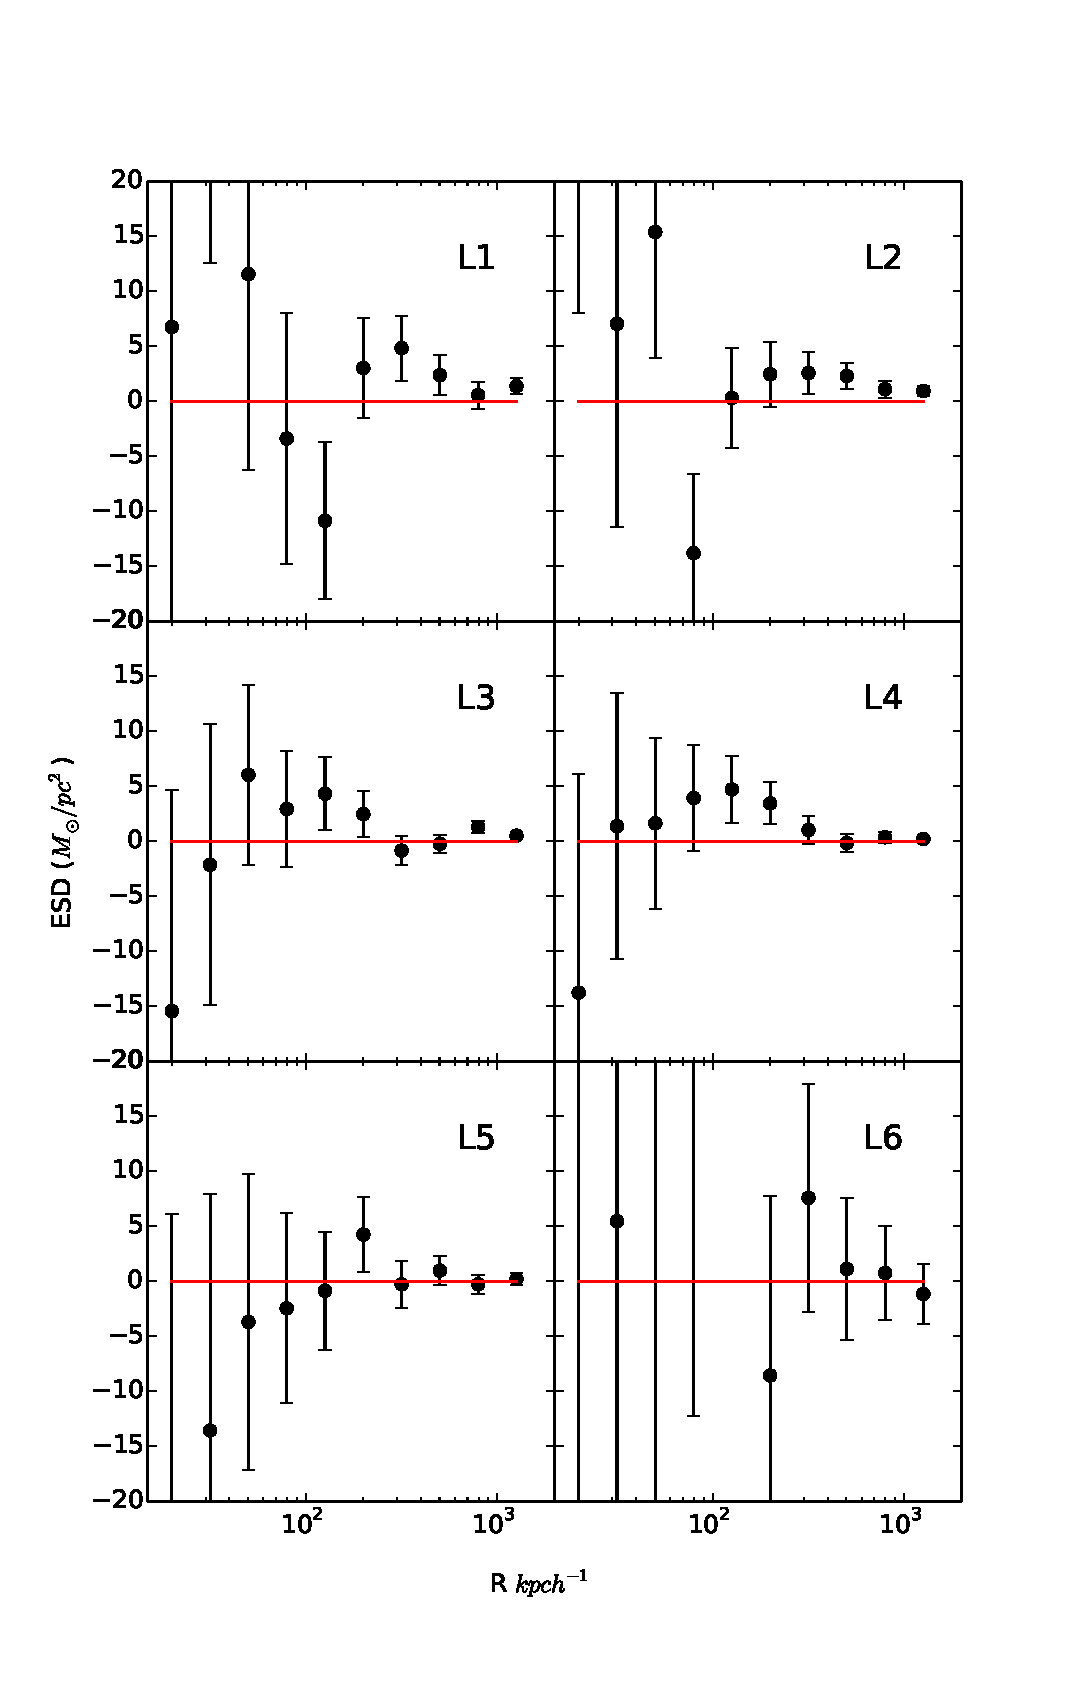
\includegraphics[width=7cm,height=9cm]{f12.eps}
\caption{The random sample check. Shown in the plot are the ESDs
  estimated around random lens galaxies.}
  \label{fig:test2}
\end{figure}


\subsubsection{45 degree rotation test}

Finally, we calculate the B mode signal using all the galaxies as did
in M05, which calculate the 45 rotated signals with 4 distance bins,
i.e., $30 <R<100\kpch$, $100 <R<600\kpch$, $600<R<2000\kpch$ and $30
<R<2000\kpch$.  Again, this systematic is consistent with zero within
one sigma error.

\begin{table}[h!]
\begin{center}
\caption{\label{tab:tbl-3} This table shows the results
   of 45 degree rotation tests as in M05. }
\begin{tabular}{ccc}
\hline
Radial range($\kpch$) & $\Delta\Sigma_{45}(hM_{\odot}{\rm pc}^{-2})$ & $\sigma_{45}$\\
\hline
$30<R<100$   & -0.46  & 1.42    \\
$100<R<600$  & 0.02   & 0.24    \\
$600<R<2000$ & -0.01  & 0.10    \\
$30<R<2000$  & -0.11  & 0.12    \\
\hline
\end{tabular}
\end{center}
\end{table}

\section{C. The ESDs of lens galaxies}

Here we provide the related ESDs measured for our SDSS DR7 lens
galaxies that are separated in different luminosity and stellar mass
bins in the following two tables. Additional ESDs for galaxies that
are separated into color and star formation subsamples, together with
$all$ the related covariance matrixes are provided in electronic files
which are available via the link
(\href{url}{http://gax.shao.ac.cn/wtluo/weak\_lensing/wl\_sdss\_dr7.tar}).

\begin{table}[h!]
\begin{center}
 \caption{\label{tab:ESD-L6} This table lists the ESDs of lens
   galaxies that are separated into different luminosity bins}.
\begin{tabular}{cccccccc}
\hline
$R Mpc/h$ & L1 & L2 & L3 & L4 & L5 & L6 \\
\hline
0.020 & $47.753 \pm 51.318$  & $22.722 \pm 31.109$   & $59.068 \pm 21.041$    & $85.001 \pm 17.596$  & $270.283 \pm 19.675$   & $395.426 \pm 112.376$  \\
0.032 & $50.609 \pm 29.971$  & $29.589 \pm 19.232$   & $28.174 \pm 13.808$    & $59.956 \pm 12.268$  & $58.845  \pm 15.307$   & $199.987 \pm 50.518 $  \\
0.050 & $27.104 \pm 18.650$  & $6.401  \pm 12.476$   & $35.059 \pm 8.693 $    & $33.181 \pm 7.948 $  & $54.852  \pm 12.084$   & $96.381  \pm 45.461 $  \\
0.080 & $0.760  \pm 11.775$  & $8.969  \pm 7.692 $   & $18.018 \pm 5.313 $    & $27.231 \pm 5.129 $  & $35.538  \pm 8.089 $   & $111.051 \pm 31.248 $  \\
0.126 & $6.225  \pm 7.465 $  & $8.183  \pm 5.040 $   & $9.380  \pm 3.491 $    & $12.053 \pm 3.055 $  & $21.476  \pm 4.981 $   & $105.765 \pm 22.670 $  \\
0.200 & $7.674  \pm 4.772 $  & $6.517  \pm 3.260 $   & $12.707 \pm 2.162 $    & $11.417 \pm 1.920 $  & $17.160  \pm 3.042 $   & $54.225  \pm 13.056 $  \\
0.317 & $3.839  \pm 3.063 $  & $3.512  \pm 1.990 $   & $4.422  \pm 1.381 $    & $8.229  \pm 1.269 $  & $14.231  \pm 1.957 $   & $38.240  \pm 8.547  $  \\
0.502 & $1.463  \pm 1.929 $  & $5.645  \pm 1.282 $   & $4.528  \pm 0.860 $    & $4.891  \pm 0.783 $  & $11.296  \pm 1.183 $   & $18.851  \pm 4.931  $  \\
0.796 & $2.557  \pm 1.266 $  & $4.166  \pm 0.797 $   & $4.106  \pm 0.551 $    & $3.616  \pm 0.526 $  & $5.322   \pm 0.758 $   & $17.179  \pm 3.135  $  \\
1.261 & $4.227  \pm 0.773 $  & $3.990  \pm 0.561 $   & $3.191  \pm 0.358 $    & $2.979  \pm 0.333 $  & $4.735   \pm 0.499 $   & $10.577  \pm 1.931  $  \\
\hline
\end{tabular}
\end{center}
\end{table}
 
\begin{table}[h!]
\begin{center}
 \caption{\label{tab:ESD-sm7} This table lists the ESDs of lens
   galaxies that are separated into different stellar mass bins}.
\begin{tabular}{ccccccccc}
\hline
$R Mpc/h$ & sm1 & sm2 & sm3 & sm4 & sm5 & sm6 & sm7 \\
\hline
0.020 & $-4.333 \pm 37.732$  & $32.952 \pm 31.256$   & $82.383 \pm 21.056$    & $182.637 \pm 21.271$  & $335.980 \pm 33.494$   & $336.404 \pm 30.651$ & $115.285 \pm 99.517$ \\
0.032 & $36.117 \pm 25.027$  & $-14.994\pm 19.186$   & $41.799 \pm 14.208$    & $91.604  \pm 15.367$  & $43.176  \pm 21.400$   & $31.518 \pm 22.789$ & $256.227 \pm 58.129 $ \\
0.050 & $16.766 \pm 15.203$  & $30.626 \pm 12.198$   & $34.166 \pm 9.904 $    & $44.174  \pm 11.545$  & $73.646  \pm 18.962$   & $66.753 \pm 18.781$ & $123.575 \pm 45.973 $ \\
0.080 & $21.305 \pm 9.069 $  & $10.033 \pm 7.549 $   & $20.878 \pm 5.701 $    & $33.090  \pm 7.798 $  & $52.717  \pm 12.550$   & $49.856 \pm 13.153$ & $113.419 \pm 35.431 $ \\
0.126 & $10.617 \pm 5.837 $  & $13.010 \pm 4.850 $   & $5.807  \pm 3.915 $    & $23.703  \pm 4.843 $  & $38.787  \pm 8.170 $   & $40.202 \pm 7.755 $ & $114.243 \pm 25.088 $ \\
0.200 & $7.286  \pm 3.841 $  & $12.030 \pm 3.186 $   & $14.715 \pm 2.401 $    & $12.398  \pm 2.847 $  & $24.732  \pm 4.965 $   & $23.755 \pm 4.770 $ & $65.843 \pm 15.455 $ \\
0.317 & $3.062  \pm 2.413 $  & $3.039  \pm 1.921 $   & $9.233  \pm 1.482 $    & $9.110   \pm 1.803 $  & $22.772  \pm 3.356 $   & $22.250 \pm 3.147 $ & $43.172 \pm 9.255 $ \\
0.502 & $3.836  \pm 1.496 $  & $3.722  \pm 1.273 $   & $5.069  \pm 0.965 $    & $9.217   \pm 1.174 $  & $15.316  \pm 2.050 $   & $14.874 \pm 1.904 $ & $22.356 \pm 5.645 $ \\
0.796 & $2.573  \pm 0.975 $  & $3.312  \pm 0.817 $   & $3.807  \pm 0.605 $    & $4.872   \pm 0.726 $  & $7.290   \pm 1.218 $   & $7.172 \pm  1.273 $ & $21.094 \pm 3.776 $ \\
1.262 & $2.929  \pm 0.570 $  & $3.503  \pm 0.497 $   & $3.155  \pm 0.383 $    & $4.023   \pm 0.480 $  & $5.760   \pm 0.786 $   & $5.703 \pm 0.749 $ & $12.316  \pm 2.337 $ \\
\hline
\end{tabular}
\end{center}
\end{table}




%




%\bibliography{ms}

\begin{thebibliography}{}

 \bibitem[Abazajian et al.(2009)]{Abazajian2009} Abazajian, K.~N.,
 Adelman-McCarthy, J.~K., Ag{\"u}eros, M.~A., et al.\ 2009, \apjs, 182, 543

\bibitem[Alam et al.(2015)]{Alam2015} Alam, S., Albareti, F.~D.,
Allende Prieto, C., et al.\ 2015, arXiv:1501.00963

 \bibitem[Amara et al.(2006)]{Amara2006} Amara, A., Metcalf,
  R.~B., Cox, T.~J., \& Ostriker, J.~P.\ 2006, \mnras, 367, 1367

 \bibitem[Amara \& R{\'e}fr{\'e}gier(2007)]{Amara2007}
  Amara, A., \& R{\'e}fr{\'e}gier, A.\ 2007, \mnras, 381, 1018

 \bibitem[Bacon \& Taylor(2003)]{Bacon2003}
 Bacon, D.~J., \& Taylor, A.~N.\ 2003, \mnras, 344, 1307

 \bibitem[Bell et al.(2003)]{Bell2003} Bell, E.~F., McIntosh,
D.~H., Katz, N., \& Weinberg, M.~D.\ 2003, \apjs, 149, 289

 \bibitem[Bartelmann \& Schneider(2001)]{Bartelman2001}
  Bartelmann, M., \& Schneider, P.\ 2001, \physrep, 340, 291

 \bibitem[Bernstein \& Jarvis(2002)]{Bernstein2002}
   Bernstein, G.~M., \& Jarvis, M.\ 2002, \aj, 123, 583

 \bibitem[Bernstein(2009)]{Bernstein2009} Bernstein, G.~M.\ 2009,
   \apj, 695, 652

 \bibitem[Bernstein \& Armstrong(2014)]{Bernstein2014}
  Bernstein, G.~M., \& Armstrong, R.\ 2014, \mnras, 438, 1880

 \bibitem[Bertin \& Arnouts(1996)]{Bertin1996}
 Bertin, E., \& Arnouts, S.\ 1996, \aaps, 117, 393

\bibitem[Blanton et al.(2003)]{Blanton2003} Blanton, M.~R.,
Brinkmann, J., Csabai, I., et al.\ 2003, \aj, 125, 2348


 \bibitem[Blanton et al.(2005)]{Blanton2005} Blanton, M.~R.,
   Schlegel, D.~J., Strauss, M.~A., et al.\ 2005, \aj, 129, 2562


 \bibitem[Bridle et al.(2002)]{Bridle2002} Bridle, S.~L., Kneib,
J.-P., Bardeau, S.,
\& Gull, S.~F.\ 2002, The Shapes of Galaxies and their Dark Halos, 38

 \bibitem[Bridle et al.(2009)]{Bridle2009} Bridle, S.,
Shawe-Taylor, J., Amara, A., et al.\ 2009, Annals of Applied Statistics, 3,6

 \bibitem[Broadhurst et al.(2005)]{Broadhurst2005} Broadhurst, T.,
  Ben{\'{\i}}tez, N., Coe, D., et al.\ 2005, \apj, 621, 53


 \bibitem[Cabanac et al.(2006)]{Cabanac2006} Cabanac, R.~A., Fort,
  B., Gavazzi, R., \& Sl2S Team 2006, SF2A-2006: Semaine de l'Astrophysique Francaise, 329


 \bibitem[Cabanac et al.(2007)]{Cabanac2007} Cabanac,
  R.~A., Alard, C., Dantel-Fort, M., et al.\ 2007, \aap, 461, 813

 \bibitem[Cacciato et al.(2009)]{Cacciato2009} Cacciato, M., van den
  Bosch, F.~C., More, S., et al.\ 2009, \mnras, 394, 929

 \bibitem[Chae(2003)]{Chae2003} Chae, K.-H.\ 2003, \mnras, 346,
   746

 \bibitem[Covone et al.(2006)]{Covone2006} Covone, G.,
  Kneib, J.-P., Soucail, G., et al.\ 2006, \aap, 456, 409

\bibitem[Cropper et al.(2013)]{Cropper2013} Cropper, M., Hoekstra,
H., Kitching, T., et al.\ 2013, \mnras, 431, 3103


 \bibitem[Csabai et al.(2003)]{2003AJ....125..580C} Csabai, I.,
   Budav{\'a}ri, T., Connolly, A.~J., et al.\ 2003, \aj, 125, 580

 \bibitem[Dalal et al.(2005)]{Dalal2005} Dalal, N., Hennawi,
  J.~F., Holder, G., \& Bode, P.\ 2005, Gravitational Lensing Impact on Cosmology, 225, 193

 \bibitem[Fischer et al.(2000)]{Fischer2000} Fischer, P., McKay,
T.~A., Sheldon, E., et al.\ 2000, \aj, 120, 1198

 \bibitem[Fu et al.(2008)]{Fu2008} Fu, L.,
  Semboloni, E., Hoekstra, H., et al.\ 2008, \aap, 479, 9

 \bibitem[George et al.(2012)]{George2012} George, M.~R.,
  Leauthaud, A., Bundy, K., et al.\ 2012, \apj, 757, 2

 \bibitem[Griffiths et al.(1996)]{Griffiths1996} Griffiths, R.~E.,
  Casertano, S., Im, M., \& Ratnatunga, K.~U.\ 1996, \mnras, 282, 1159

 \bibitem[Gunn et al.(1998)]{Gunn1998} Gunn, J.~E., Carr, M.,
  Rockosi, C., et al.\ 1998, \aj, 116, 3040

 \bibitem[Hamilton \& Tegmark(2004)]{Hamilton2004}
 Hamilton, A.~J.~S., \& Tegmark, M.\ 2004, \mnras, 349, 115

 \bibitem[Heymans et al.(2004)]{Heymans2004} Heymans, C., Brown, M.,
  Heavens, A., et al.\ 2004, \mnras, 347, 895

 \bibitem[Heymans et al.(2005)]{Heymans2005} Heymans, C., Brown,
  M.~L., Barden, M., et al.\ 2005, \mnras, 361, 160

  \bibitem[Heymans et al.(2006)]{Heymans2006} Heymans, C., Van
Waerbeke, L., Bacon, D., et al.\ 2006, \mnras, 368, 1323

 \bibitem[Heymans et al.(2012)]{Heymans2012} Heymans, C., Van
  Waerbeke, L., Miller, L., et al.\ 2012, \mnras, 427, 146

 \bibitem[Hirata \& Seljak(2003)]{Hirata2003}
  Hirata, C., \& Seljak, U.\ 2003, \mnras, 343, 459
  
 \bibitem[Hirata et al.(2004)]{Hirata2004} Hirata, C.~M., 
Mandelbaum, R., Seljak, U., et al.\ 2004, \mnras, 353, 529 

 \bibitem[Hirata et al.(2008)]{Hirata2008} Hirata, C.~M., Ho, S.,
  Padmanabhan, N., Seljak, U., \& Bahcall, N.~A.\ 2008, \prd, 78, 043520

 \bibitem[Hoekstra et al.(2000)]{Hoekstra2000} Hoekstra, H., Franx,
M., \& Kuijken, K.\ 2000, \apj, 532, 88

 \bibitem[Hoekstra et al.(1998)]{Hoekstra1998} Hoekstra, H., Franx,
  M., Kuijken, K., \& Squires, G.\ 1998, \apj, 504, 636

 \bibitem[Hoekstra \& Jain(2008)]{Hoekstra2008} Hoekstra, H.,
  \& Jain, B.\ 2008, Annual Review of Nuclear and Particle Science, 58, 99

 \bibitem[Kaifu(1998)]{Kaifu1998} Kaifu, N.\ 1998, \procspie,
  3352, 14

 \bibitem[Kaiser et al.(1995)]{Kaiser1995} Kaiser, N., Squires, G.,
   \& Broadhurst, T.\ 1995, \apj, 449, 460

  \bibitem[Kaiser(2000)]{Kaiser2000} Kaiser, N.\ 2000, \apj, 537,
555

\bibitem[Kauffmann et al.(2003)]{Kauffmann2003} Kauffmann, G.,
Heckman, T.~M., White, S.~D.~M., et al.\ 2003, \mnras, 341, 33

 \bibitem[Kitching et al.(2008)]{Kitching2008} Kitching, T.~D.,
  Miller, L., Heymans, C.~E., van Waerbeke, L.,
  \& Heavens, A.~F.\ 2008, \mnras, 390, 149

 \bibitem[Kitching et al.(2010)]{Kitching2010} Kitching, T., Balan,
S., Bernstein, G., et al.\ 2010, arXiv:1009.0779

 \bibitem[Kilbinger et al.(2013)]{Kilbinger2013} Kilbinger, M., Fu,
  L., Heymans, C., et al.\ 2013, \mnras, 430, 2200

 \bibitem[Kneib et al.(2004)]{Kneib2004} Kneib, J.-P., Ellis,
  R.~S., Santos, M.~R., \& Richard, J.\ 2004, \apj, 607, 697

 \bibitem[Kneib(2006)]{Kneib2006} Kneib, J.-P.\ 2006, HST
  Proposal, 10876

\bibitem[Koekemoer et al.(2007)]{Koekemoer2007} Koekemoer, A.~M.,
Aussel, H., Calzetti, D., et al.\ 2007, \apjs, 172, 196

\bibitem[Kuijken et al.(2015)]{Kuijken2015} Kuijken, K., Heymans, 
C., Hildebrandt, H., et al.\ 2015, \mnras, 454, 3500 


\bibitem[Leauthaud et al.(2007)]{Leauthaud2007} Leauthaud, A.,
Massey, R., Kneib, J.-P., et al.\ 2007, \apjs, 172, 219


 \bibitem[Leauthaud et al.(2012)]{Leauthaud2012} Leauthaud, A.,
  Tinker, J., Bundy, K., et al.\ 2012, \apj, 744, 159

 \bibitem[Li et al.(2009)]{Li2009} Li, R., Mo, H.~J., Fan, Z.,
  et al.\ 2009, \mnras, 394, 1016

 \bibitem[Li et al.(2013)]{Li2013} Li, R., Mo, H.~J., Fan, Z.,
Yang, X., \& Bosch, F.~C.~v.~d.\ 2013, \mnras, 430, 3359


 \bibitem[Li et al.(2014)]{Li2014} Li, R., Shan, H., Mo, H., et
  al.\ 2014, \mnras, 438, 2864


 \bibitem[Liu et al.(2014)]{Liu2014} Liu, X., Pan, C., Li, R.,
  et al.\ 2014, arXiv:1412.3683
  
  \bibitem[LSST Science Collaboration et al.(2009)]{LSST2009} LSST 
Science Collaboration, Abell, P.~A., Allison, J., et al.\ 2009, 
arXiv:0912.0201 


\bibitem[Luo et al.(2014)]{Luo2014} Luo, W., Yang, X.,
\& Zhang, Y.\ 2014, \apjl, 789, L16


 \bibitem[Lupton et al.(2001)]{Lupton2001} Lupton, R., Gunn, J.~E.,
Ivezi{\'c}, Z., Knapp, G.~R.,
\& Kent, S.\ 2001, Astronomical Data Analysis Software and Systems X, 238, 269

\bibitem[Jarvis et al.(2015)]{Jarvis2015} Jarvis, M., Sheldon, E., 
Zuntz, J., et al.\ 2015, arXiv:1507.05603 


 \bibitem[Mandelbaum et al.(2005)]{Mandelbaum2005} Mandelbaum, R.,
  Hirata, C.~M., Seljak, U., et al.\ 2005, \mnras, 361, 1287


\bibitem[Mandelbaum et al.(2006)]{Mandelbaum2006} Mandelbaum, R.,
  Seljak, U., Kauffmann, G., Hirata, C.~M., \& Brinkmann, J.\ 2006,
  \mnras, 368, 715


 \bibitem[Mandelbaum et al.(2008)]{Mandelbaum2008} Mandelbaum, R.,
  Seljak, U., Hirata, C.~M., et al.\ 2008, \mnras, 386, 781

 \bibitem[Mandelbaum et al.(2009a)]{Mandelbaum2009a} Mandelbaum, R., van
  de Ven, G., \& Keeton, C.~R.\ 2009a, \mnras, 398, 635


 \bibitem[Mandelbaum et al.(2009b)]{Mandelbaum2009b} Mandelbaum, R., Li,
  C., Kauffmann, G., \& White, S.~D.~M.\ 2009b, \mnras, 393, 377


 \bibitem[Mandelbaum et al.(2012)]{Mandelbaum2012} Mandelbaum, R.,
Hirata, C.~M., Leauthaud, A., Massey, R.~J.,
\& Rhodes, J.\ 2012, \mnras, 420, 1518

 \bibitem[Mandelbaum et al.(2013)]{Mandelbaum2013} Mandelbaum, R.,
  Slosar, A., Baldauf, T., et al.\ 2013, \mnras, 432, 1544

 \bibitem[Mandelbaum et al.(2014)]{Mandelbaum2014} Mandelbaum, R.,
  Rowe, B., Bosch, J., et al.\ 2014, \apjs, 212, 5

\bibitem[Mandelbaum et al.(2015)]{Mandelbaum2015} Mandelbaum, R., 
Rowe, B., Armstrong, R., et al.\ 2015, \mnras, 450, 2963 


 \bibitem[Maoli et al.(2000)]{Maoli2000} Maoli, R., Mellier, Y.,
  van Waerbeke, L., et al.\ 2000, The Messenger, 101, 10

 \bibitem[Massey \& Refregier(2005)]{Massey2005}
 Massey, R., \& Refregier, A.\ 2005, \mnras, 363, 197

 \bibitem[Massey et al.(2007a)]{Massey2007} Massey, R., Rhodes, J.,
  Leauthaud, A., et al.\ 2007a, \apjs, 172, 239

\bibitem[Massey et al.(2007b)]{Massey2007b} Massey, R., Heymans, C.,
Berg{\'e}, J., et al.\ 2007b, \mnras, 376, 13

\bibitem[Massey et al.(2010)]{Massey2010} Massey, R., Stoughton,
C., Leauthaud, A., et al.\ 2010, \mnras, 401, 371

\bibitem[Massey et al.(2013)]{Massey2013} Massey, R., Hoekstra,
H., Kitching, T., et al.\ 2013, \mnras, 429, 661

\bibitem[Miller et al.(2007)]{Miller2007} Miller, L., Kitching,
T.~D., Heymans, C., Heavens, A.~F., \& van Waerbeke, L.\ 2007, \mnras, 382, 315

 \bibitem[Miller et al.(2013)]{Miller2013} Miller, L., Heymans, C.,
  Kitching, T.~D., et al.\ 2013, \mnras, 429, 2858

 \bibitem[Mo et al.(2010)]{2010gfe..book.....M} Mo, H., van den Bosch, F.~C.,
   \& White, S.\ 2010, Galaxy Formation and Evolution.~Cambridge University
   Press, 2010.~ISBN: 9780521857932

 \bibitem[Motohara et al.(2005)]{Motohara2005} Motohara, K., Takata,
  T., Iwamuro, F., et al.\ 2005, \aj, 129, 53

 \bibitem[Nakajima \& Bernstein(2007)]{Nakajima2007}
   Nakajima, R., \& Bernstein, G.\ 2007, \aj, 133, 1763

 \bibitem[Navarro et al.(1997)]{NFW1997} Navarro, J.~F., Frenk,
  C.~S., \& White, S.~D.~M.\ 1997, \apj, 490, 493

 \bibitem[Oguri et al.(2002)]{Oguri2002} Oguri, M., Taruya, A.,
   Suto, Y., \& Turner, E.~L.\ 2002, \apj, 568, 488

 \bibitem[Oguri et al.(2009)]{Oguri2009} Oguri, M., Hennawi,
J.~F., Gladders, M.~D., et al.\ 2009, \apj, 699, 1038

 \bibitem[Oguri et al.(2010)]{Oguri2010} Oguri, M., Takada, M.,
Okabe, N., \& Smith, G.~P.\ 2010, \mnras, 405, 2215

 \bibitem[Okabe et al.(2014)]{Okabe2014} Okabe, N., Futamase, T.,
  Kajisawa, M., \& Kuroshima, R.\ 2014, \apj, 784, 90

 \bibitem[Refregier(2003)]{Refregier2003} Refregier, A.\ 2003, \araa, 41, 645
 
 \bibitem[Refregier et al.(2010)]{Refregier2010} Refregier, A., Amara, 
A., Kitching, T.~D., et al.\ 2010, arXiv:1001.0061 

 \bibitem[Rhodes et al.(2000)]{Rhodes2000} Rhodes, J., Refregier,
A., \& Groth, E.~J.\ 2000, \apj, 536, 79

 \bibitem[Rhodes et al.(2007)]{Rhodes2007} Rhodes, J.~D., Massey,
  R.~J., Albert, J., et al.\ 2007, \apjs, 172, 203

\bibitem[Rowe et al.(2015)]{Rowe2015} Rowe, B.~T.~P.,
Jarvis, M., Mandelbaum, R., et al.\ 2015, Astronomy and Computing, 10, 121


\bibitem[Scoville et al.(2007a)]{Scoville2007a} Scoville, N., Abraham,
R.~G., Aussel, H., et al.\ 2007a, \apjs, 172, 38


\bibitem[Scoville et al.(2007b)]{Scoville2007b} Scoville, N., Aussel,
H., Brusa, M., et al.\ 2007b, \apjs, 172, 1


 \bibitem[Sheldon et al.(2004)]{Sheldon2004} Sheldon, E.~S.,
  Johnston, D.~E., Frieman, J.~A., et al.\ 2004, \aj, 127, 2544

 \bibitem[Sheldon et al.(2009)]{Sheldon2009} Sheldon, E.~S.,
  Johnston, D.~E., Scranton, R., et al.\ 2009, \apj, 703, 2217


 \bibitem[Simet et al.(2012)]{Simet2012} Simet, M., Kubo, J.~M.,
  Dodelson, S., et al.\ 2012, \apj, 748, 128

  \bibitem[Strauss et al.(2002)]{Strass2002} Strauss, M.~A.,
Weinberg, D.~H., Lupton, R.~H., et al.\ 2002, \aj, 124, 1810

 \bibitem[Tortora(2007)]{Tortora2007} Tortora, C.\ 2007, 1st
  Workshop of Astronomy and Astrophysics for Students, 127



\bibitem[Treu et al.(2006)]{Treu2006} Treu, T., Koopmans, L.~V.,
  Bolton, A.~S., Burles, S., \& Moustakas, L.~A.\ 2006, \apj, 640, 662


 \bibitem[Umetsu et al.(2005)]{Umetsu2005} Umetsu, K., Tanaka, M.,
  Kodama, T., et al.\ 2005, \pasj, 57, 877

 \bibitem[Umetsu(2007)]{Umetsu2007} Umetsu, K.\ 2007, Subaru
  Proposal, 24

 \bibitem[Umetsu et al.(2014)]{Umetsu2014} Umetsu, K., Medezinski,
  E., Nonino, M., et al.\ 2014, \apj, 795, 163

 \bibitem[van den Bosch et al.(2004)]{Bosch2004} van den Bosch,
  F.~C., Norberg, P., Mo, H.~J., \& Yang, X.\ 2004, \mnras, 352, 1302

 \bibitem[van Waerbeke(2001)]{vanWaerbeke2001} van Waerbeke, L.\ 2001,
Cosmological Physics with Gravitational Lensing, 165

 \bibitem[Walsh et al.(1979)]{Walsh1979} Walsh, D., Wills, B.~J.,
  \& Wills, D.\ 1979, \mnras, 189, 667


 \bibitem[Wang et al.(2014)]{Wang2014} Wang, L., Yang, X., Shen,
  S., et al.\ 2014, \mnras, 439, 611
  
  \bibitem[Wittman et al.(2006)]{Wittman2006} Wittman, D., 
Dell'Antonio, I.~P., Hughes, J.~P., et al.\ 2006, \apj, 643, 128 



 \bibitem[Yang et al.(2003)]{Yang2003} Yang, X.~H., Mo, H.~J.,
Kauffmann, G., \& Chu, Y.~Q.\ 2003, \mnras, 339, 387


\bibitem[Yang et al.(2006a)]{Yang2006a} Yang, X., Mo, H.~J., van
den Bosch, F.~C., et al.\ 2006a, \mnras, 373, 1159


\bibitem[Yang et al.(2006b)]{Yang2006b} Yang, X., Mo, H.~J.,
\& van den Bosch, F.~C.\ 2006b, \apjl, 638, L55


 \bibitem[Yang et al.(2007)]{Yang2007} Yang, X., Mo, H.~J., van
 den Bosch, F.~C., et al.\ 2007, \apj, 671, 153

 \bibitem[Yang et al.(2008)]{Yang2008} Yang, X., Mo, H.~J.,
   \& van den Bosch, F.~C.\ 2008, \apj, 676, 248

\bibitem[Yang et al.(2012)]{Yang2012} Yang, X., Mo, H.~J., van den
  Bosch, F.~C., Zhang, Y., \& Han, J.\ 2012, \apj, 752, 41

 \bibitem[Yang et al.(2013)]{Yang2013} Yang, X., Mo, H.~J., van den
   Bosch, F.~C., et al.\ 2013, \apj, 770, 115


 \bibitem[York et al.(2000)]{York2000} York, D.~G., Adelman, J.,
 Anderson, J.~E., Jr., et al.\ 2000, \aj, 120, 1579

  \bibitem[Zhang (2010)]{Zhang2010} Zhang, J.\ 2010, \mnras, 403,
 673

 \bibitem[Zhang (2011)]{Zhang2011} Zhang, J.\ 2011, JCAP, 11, 041


 \bibitem[Zhang et al.(2015)]{Zhang2015} Zhang, J., Luo, W.,
  \& Foucaud, S.\ 2015, JCAP, 1, 024


\bibitem[Zu et al.(2014)]{Zu2014} Zu, Y., Weinberg, D.~H.,
  Jennings, E., Li, B., \& Wyman, M.\ 2014, \mnras, 445, 1885

 \bibitem[Zu \& Weinberg(2013)]{Zu2013} Zu, Y.,
  \& Weinberg, D.~H.\ 2013, \mnras, 431, 3319


\end{thebibliography}

\end{document}


